% !Rnw weave = knitr
%\VignetteEngine{knitr::knitr}
%\VignetteIndexEntry{Tutorial: Working with categorical data with R and the vcd package}
%\VignetteDepends{vcd,gmodels,ca,gnm}
%\VignetteKeywords{contingency tables, mosaic plots, sieve plots, categorical data, independence, conditional independence, R}
%\VignettePackage{vcdExtra}

\documentclass[10pt,twoside]{article}\usepackage[]{graphicx}\usepackage[]{color}
%% maxwidth is the original width if it is less than linewidth
%% otherwise use linewidth (to make sure the graphics do not exceed the margin)
\makeatletter
\def\maxwidth{ %
  \ifdim\Gin@nat@width>\linewidth
    \linewidth
  \else
    \Gin@nat@width
  \fi
}
\makeatother

\definecolor{fgcolor}{rgb}{0.345, 0.345, 0.345}
\newcommand{\hlnum}[1]{\textcolor[rgb]{0.686,0.059,0.569}{#1}}%
\newcommand{\hlstr}[1]{\textcolor[rgb]{0.192,0.494,0.8}{#1}}%
\newcommand{\hlcom}[1]{\textcolor[rgb]{0.678,0.584,0.686}{\textit{#1}}}%
\newcommand{\hlopt}[1]{\textcolor[rgb]{0,0,0}{#1}}%
\newcommand{\hlstd}[1]{\textcolor[rgb]{0.345,0.345,0.345}{#1}}%
\newcommand{\hlkwa}[1]{\textcolor[rgb]{0.161,0.373,0.58}{\textbf{#1}}}%
\newcommand{\hlkwb}[1]{\textcolor[rgb]{0.69,0.353,0.396}{#1}}%
\newcommand{\hlkwc}[1]{\textcolor[rgb]{0.333,0.667,0.333}{#1}}%
\newcommand{\hlkwd}[1]{\textcolor[rgb]{0.737,0.353,0.396}{\textbf{#1}}}%

\usepackage{framed}
\makeatletter
\newenvironment{kframe}{%
 \def\at@end@of@kframe{}%
 \ifinner\ifhmode%
  \def\at@end@of@kframe{\end{minipage}}%
  \begin{minipage}{\columnwidth}%
 \fi\fi%
 \def\FrameCommand##1{\hskip\@totalleftmargin \hskip-\fboxsep
 \colorbox{shadecolor}{##1}\hskip-\fboxsep
     % There is no \\@totalrightmargin, so:
     \hskip-\linewidth \hskip-\@totalleftmargin \hskip\columnwidth}%
 \MakeFramed {\advance\hsize-\width
   \@totalleftmargin\z@ \linewidth\hsize
   \@setminipage}}%
 {\par\unskip\endMakeFramed%
 \at@end@of@kframe}
\makeatother

\definecolor{shadecolor}{rgb}{.97, .97, .97}
\definecolor{messagecolor}{rgb}{0, 0, 0}
\definecolor{warningcolor}{rgb}{1, 0, 1}
\definecolor{errorcolor}{rgb}{1, 0, 0}
\newenvironment{knitrout}{}{} % an empty environment to be redefined in TeX

\usepackage{alltt}

\usepackage{bm}
\usepackage[toc]{multitoc}   % for table of contents

% from Z.cls
\usepackage[authoryear,round,longnamesfirst]{natbib}
\bibpunct{(}{)}{;}{a}{}{,}
\bibliographystyle{jss}

\usepackage{hyperref}
\usepackage{color}
%% colors
\definecolor{Red}{rgb}{0.7,0,0}
\definecolor{Blue}{rgb}{0,0,0.8}
\hypersetup{%
  hyperindex = {true},
  colorlinks = {true},
%  linktocpage = {true},
  plainpages = {false},
  linkcolor = {Blue},
  citecolor = {Blue},
  urlcolor = {Red},
  pdfstartview = {Fit},
  pdfpagemode = {UseOutlines},
  pdfview = {XYZ null null null}
}
%\AtBeginDocument{
%  \hypersetup{%
%    pdfauthor = {Michael Friendly},
%    pdftitle = {Tutorial: Working with categorical data with R and the vcd package},
%    pdfkeywords = {contingency tables, mosaic plots, sieve plots, categorical data, independence, conditional independence, R}
%  }
%}


% math stuff
\newcommand*{\given}{\ensuremath{\, | \,}}
\renewcommand*{\vec}[1]{\ensuremath{\bm{#1}}}
\newcommand{\mat}[1]{\ensuremath{\bm{#1}}}
\newcommand{\trans}{\ensuremath{^\mathsf{T}}}
\newcommand{\diag}[1]{\ensuremath{\mathrm{diag} (#1)}}
\def\binom#1#2{{#1 \choose #2}}%
\newcommand{\implies}{ \ensuremath{\mapsto} }

\newenvironment{equation*}{\displaymath}{\enddisplaymath}%

\newcommand{\tabref}[1]{Table~\ref{#1}}
\newcommand{\figref}[1]{Figure~\ref{#1}}
\newcommand{\secref}[1]{Section~\ref{#1}}
\newcommand{\loglin}{loglinear }

%\usepackage{thumbpdf}

% page dimensions
\addtolength{\hoffset}{-1.5cm}
\addtolength{\textwidth}{3cm}
\addtolength{\voffset}{-1cm}
\addtolength{\textheight}{2cm}

% Vignette examples
\newcommand*{\Example}{\fbox{\textbf{\emph{Example}}:} }

% R stuff
\newcommand{\var}[1]{\textit{\texttt{#1}}}
\newcommand{\data}[1]{\texttt{#1}}
\newcommand{\class}[1]{\textsf{"#1"}}
%% \code without `-' ligatures
\def\nohyphenation{\hyphenchar\font=-1 \aftergroup\restorehyphenation}
\def\restorehyphenation{\hyphenchar\font=`-}
{\catcode`\-=\active%
  \global\def\code{\bgroup%
    \catcode`\-=\active \let-\codedash%
    \Rd@code}}
\def\codedash{-\discretionary{}{}{}}
\def\Rd@code#1{\texttt{\nohyphenation#1}\egroup}

\newcommand{\codefun}[1]{\code{#1()}}
\let\proglang=\textsf
\newcommand{\pkg}[1]{{\normalfont\fontseries{b}\selectfont #1}}
\newcommand{\Rpackage}[1]{{\textsf{#1}}}

%% almost as usual
\author{Michael Friendly\\York University, Toronto}
\title{Working with categorical data with \proglang{R} and the \pkg{vcd} and \pkg{vcdExtra} packages}
\date{\footnotesize{Using \Rpackage{vcdExtra} version 0.5-11
  and \Rpackage{vcd} version 1.2-13; Date: 2013-09-05}}


%% for pretty printing and a nice hypersummary also set:
%\Plainauthor{Michael Friendly} %% comma-separated
%\Shorttitle{vcd tutorial} %% a short title (if necessary)
%\Plaintitle{Tutorial: Working with categorical data with R and the vcd package}

%\SweaveOpts{engine=R,eps=TRUE,height=6,width=7,results=hide,fig=FALSE,echo=TRUE}












%\SweaveOpts{concordance=TRUE}
\setkeys{Gin}{width=0.7\textwidth}






%% end of declarations %%%%%%%%%%%%%%%%%%%%%%%%%%%%%%%%%%%%%%%%%%%%%%%
\IfFileExists{upquote.sty}{\usepackage{upquote}}{}


\begin{document}




\maketitle

%% an abstract and keywords
\begin{abstract}
This tutorial describes the creation of frequency and contingency tables
from categorical variables, along with tests of independence, measures
of association, and methods for graphically displaying results. 
The framework is provided by the \proglang{R} package \pkg{vcd},
but other packages are used to help with various tasks.  
The \pkg{vcdExtra} package extends the graphical and statistical methods provided by
\pkg{vcd}.
\end{abstract}

%\keywords{contingency tables, mosaic plots, sieve plots, 
%categorical data, independence, conditional independence, generalized linear models,
%\proglang{R}}
%\Plainkeywords{contingency tables, mosaic plots, 
%  sieve plots, categorical data, independence, 
%  conditional independence, generalized linear models, R}

{\small
% \sloppy
% \begin{multicols}{2}
 \tableofcontents
% \end{multicols}
}


\section[Introduction]{Introduction}\label{sec:intro}
%% Note: If there is markup in \(sub)section, then it has to be escape as above.


This tutorial, part of the \pkg{vcdExtra} package,
describes how to work with categorical data in the context of
fitting statistical models in \proglang{R} and visualizing
the results using the \pkg{vcd} and \pkg{vcdExtra} packages.
It focuses first on methods and tools for creating
and manipulating \proglang{R} data objects which represent
frequency and contingency tables involving
categorical variables.

Further sections describe some simple methods for calculating 
tests of independence and measures of association amomg 
categorial variables, and also
methods for graphically displaying results.

There is much more to the analysis of categorical data than is described here,
where the emphasis is on cross-tabulated tables of frequencies (``contingency tables''),
statistical tests, associated \loglin\ models, and visualization of \emph{how}
variables are related.

A more general treatment of graphical methods for categorical data is contained
in my book, \emph{Visualizing Categorical Data} \citep{vcd:Friendly:2000}, for which
\pkg{vcd} is a partial \proglang{R} companion, covering topics not otherwise
available in \proglang{R}.  On the other hand, the implementation of graphical
methods in \pkg{vcd} is more general in many respects than what I provided in
\proglang{SAS}. Statistical models for categorical data in \proglang{R} have
been extended considerably with the \pkg{gnm} package for generalized \emph{nonlinear}
models.  The \pkg{vcdExtra} package extends \pkg{vcd} methods to models fit using
\codefun{glm} and \codefun{gnm}.

A more complete theoretical description of these statistical
methods is provided in Agresti's \citeyearpar{vcd:Agresti:2002,Agresti:2013}
\emph{Categorical Data Analysis}. For this, see
the \proglang{Splus/R} companion by Laura Thompson,
\url{https://home.comcast.net/~lthompson221/Splusdiscrete2.pdf}
and Agresti's support web page,
\url{http://www.stat.ufl.edu/~aa/cda/cda.html}.



\section[Creating frequency tables]{Creating and manipulating frequency tables}\label{sec:creating}

\proglang{R} provides many methods for creating frequency and contingency tables. Several are
described below. In the examples below, we use some real examples and some anonymous
ones, where the variables \code{A}, \code{B}, and \code{C}  represent
categorical variables, and \code{X} represents an arbitrary \proglang{R} data object.

The first thing you need to know is that categorical data can be represented in
three different forms in \proglang{R}, and it is sometimes necessary to convert
from one form to another, for carrying out statistical tests, fitting models
or visualizing the results.  Once a data object exists in \proglang{R}, 
you can examine its complete structure with
the \codefun{str} function, or view the names of its components with the
\codefun{names} function.
 
\begin{description}
  \item[case form] a data frame containing individual observations, with one or
  more factors, used as the classifying variables. In case form, there may also
  be numeric covariates. 
  The total number of observations
  is \code{nrow(X)}, and the number of variables is \code{ncol(X)}.
  	
\Example
The \data{Arthritis} data is available in case form in the \pkg{vcd} package. 
There are two explanatory factors: \code{Treatment} and \code{Sex}. \code{Age}
is a numeric covariate, and \code{Improved} is the response--- an ordered factor,
with levels 
\code{None < Some < Marked}.  
Excluding \code{Age}, we would have
a $2 \times 2 \times 3$ contingency table for \code{Treatment}, \code{Sex} and \code{Improved}.
%\code{"None" < "Some" < "Marked"}.
\begin{knitrout}
\definecolor{shadecolor}{rgb}{0.969, 0.969, 0.969}\color{fgcolor}\begin{kframe}
\begin{alltt}
\hlkwd{names}\hlstd{(Arthritis)}      \hlcom{# show the variables}
\end{alltt}
\begin{verbatim}
## [1] "ID"        "Treatment" "Sex"       "Age"       "Improved"
\end{verbatim}
\begin{alltt}
\hlkwd{str}\hlstd{(Arthritis)}        \hlcom{# show the structure}
\end{alltt}
\begin{verbatim}
## 'data.frame':	84 obs. of  5 variables:
##  $ ID       : int  57 46 77 17 36 23 75 39 33 55 ...
##  $ Treatment: Factor w/ 2 levels "Placebo","Treated": 2 2 2 2 2 2 2 2 2 2 ...
##  $ Sex      : Factor w/ 2 levels "Female","Male": 2 2 2 2 2 2 2 2 2 2 ...
##  $ Age      : int  27 29 30 32 46 58 59 59 63 63 ...
##  $ Improved : Ord.factor w/ 3 levels "None"<"Some"<..: 2 1 1 3 3 3 1 3 1 1 ...
\end{verbatim}
\begin{alltt}
\hlkwd{head}\hlstd{(Arthritis,}\hlnum{5}\hlstd{)}     \hlcom{# first 5 observations, same as Arthritis[1:5,] }
\end{alltt}
\begin{verbatim}
##   ID Treatment  Sex Age Improved
## 1 57   Treated Male  27     Some
## 2 46   Treated Male  29     None
## 3 77   Treated Male  30     None
## 4 17   Treated Male  32   Marked
## 5 36   Treated Male  46   Marked
\end{verbatim}
\end{kframe}
\end{knitrout}

  
  \item[frequency form] a data frame containing one or more factors, and a frequency 
  variable, often called \code{Freq} or \code{count}.  The total number of observations
  is 
  \verb|sum(X$Freq)|,  
  \code{sum(X[,"Freq"])} or some equivalent form.
  The number of cells in the table is \code{nrow(X)}.

\Example 
For small frequency tables, it is often convenient to enter them in frequency form
using \codefun{expand.grid} for the factors and \codefun{c} to list the counts in a vector.
The example below, from \cite{vcd:Agresti:2002} gives results for the 1991 General Social Survey,
with respondents classified by sex and party identification.
\begin{knitrout}
\definecolor{shadecolor}{rgb}{0.969, 0.969, 0.969}\color{fgcolor}\begin{kframe}
\begin{alltt}
\hlcom{# Agresti (2002), table 3.11, p. 106}
\hlstd{GSS} \hlkwb{<-} \hlkwd{data.frame}\hlstd{(}
  \hlkwd{expand.grid}\hlstd{(}\hlkwc{sex}\hlstd{=}\hlkwd{c}\hlstd{(}\hlstr{"female"}\hlstd{,} \hlstr{"male"}\hlstd{),}
              \hlkwc{party}\hlstd{=}\hlkwd{c}\hlstd{(}\hlstr{"dem"}\hlstd{,} \hlstr{"indep"}\hlstd{,} \hlstr{"rep"}\hlstd{)),}
  \hlkwc{count}\hlstd{=}\hlkwd{c}\hlstd{(}\hlnum{279}\hlstd{,}\hlnum{165}\hlstd{,}\hlnum{73}\hlstd{,}\hlnum{47}\hlstd{,}\hlnum{225}\hlstd{,}\hlnum{191}\hlstd{))}
\hlstd{GSS}
\end{alltt}
\begin{verbatim}
##      sex party count
## 1 female   dem   279
## 2   male   dem   165
## 3 female indep    73
## 4   male indep    47
## 5 female   rep   225
## 6   male   rep   191
\end{verbatim}
\begin{alltt}
\hlkwd{names}\hlstd{(GSS)}
\end{alltt}
\begin{verbatim}
## [1] "sex"   "party" "count"
\end{verbatim}
\begin{alltt}
\hlkwd{str}\hlstd{(GSS)}
\end{alltt}
\begin{verbatim}
## 'data.frame':	6 obs. of  3 variables:
##  $ sex  : Factor w/ 2 levels "female","male": 1 2 1 2 1 2
##  $ party: Factor w/ 3 levels "dem","indep",..: 1 1 2 2 3 3
##  $ count: num  279 165 73 47 225 191
\end{verbatim}
\begin{alltt}
\hlkwd{sum}\hlstd{(GSS}\hlopt{$}\hlstd{count)}
\end{alltt}
\begin{verbatim}
## [1] 980
\end{verbatim}
\end{kframe}
\end{knitrout}


  \item[table form]  a matrix, array or table object, whose elements are the frequencies
  in an $n$-way table.  The variable names (factors) and their levels are given by
  \code{dimnames(X)}. The total number of observations
  is \code{sum(X)}.  The number of dimensions of the table is \code{length(dimnames(X))},
  and the table sizes are given by \code{sapply(dimnames(X), length)}.
  	
\Example 
The \data{HairEyeColor} is stored in table form in \pkg{vcd}. Examine some attributes: 
\begin{knitrout}
\definecolor{shadecolor}{rgb}{0.969, 0.969, 0.969}\color{fgcolor}\begin{kframe}
\begin{alltt}
\hlkwd{str}\hlstd{(HairEyeColor)}                      \hlcom{# show the structure}
\end{alltt}
\begin{verbatim}
##  table [1:4, 1:4, 1:2] 32 53 10 3 11 50 10 30 10 25 ...
##  - attr(*, "dimnames")=List of 3
##   ..$ Hair: chr [1:4] "Black" "Brown" "Red" "Blond"
##   ..$ Eye : chr [1:4] "Brown" "Blue" "Hazel" "Green"
##   ..$ Sex : chr [1:2] "Male" "Female"
\end{verbatim}
\begin{alltt}
\hlkwd{sum}\hlstd{(HairEyeColor)}                      \hlcom{# number of cases}
\end{alltt}
\begin{verbatim}
## [1] 592
\end{verbatim}
\begin{alltt}
\hlkwd{sapply}\hlstd{(}\hlkwd{dimnames}\hlstd{(HairEyeColor), length)} \hlcom{# table dimension sizes}
\end{alltt}
\begin{verbatim}
## Hair  Eye  Sex 
##    4    4    2
\end{verbatim}
\end{kframe}
\end{knitrout}


\Example 
Enter frequencies in a matrix, and assign \code{dimnames},
giving the variable names and category labels.  Note that, by default,
\codefun{matrix} uses the elements supplied by \emph{columns} in the
result, unless you specify \code{byrow=TRUE}.
\begin{knitrout}
\definecolor{shadecolor}{rgb}{0.969, 0.969, 0.969}\color{fgcolor}\begin{kframe}
\begin{alltt}
\hlcom{## A 4 x 4 table  Agresti (2002, Table 2.8, p. 57) Job Satisfaction}
\hlstd{JobSat} \hlkwb{<-} \hlkwd{matrix}\hlstd{(}\hlkwd{c}\hlstd{(}\hlnum{1}\hlstd{,}\hlnum{2}\hlstd{,}\hlnum{1}\hlstd{,}\hlnum{0}\hlstd{,} \hlnum{3}\hlstd{,}\hlnum{3}\hlstd{,}\hlnum{6}\hlstd{,}\hlnum{1}\hlstd{,} \hlnum{10}\hlstd{,}\hlnum{10}\hlstd{,}\hlnum{14}\hlstd{,}\hlnum{9}\hlstd{,} \hlnum{6}\hlstd{,}\hlnum{7}\hlstd{,}\hlnum{12}\hlstd{,}\hlnum{11}\hlstd{),} \hlnum{4}\hlstd{,} \hlnum{4}\hlstd{)}
\hlkwd{dimnames}\hlstd{(JobSat)} \hlkwb{=} \hlkwd{list}\hlstd{(}\hlkwc{income}\hlstd{=}\hlkwd{c}\hlstd{(}\hlstr{"< 15k"}\hlstd{,} \hlstr{"15-25k"}\hlstd{,} \hlstr{"25-40k"}\hlstd{,} \hlstr{"> 40k"}\hlstd{),}
                \hlkwc{satisfaction}\hlstd{=}\hlkwd{c}\hlstd{(}\hlstr{"VeryD"}\hlstd{,} \hlstr{"LittleD"}\hlstd{,} \hlstr{"ModerateS"}\hlstd{,} \hlstr{"VeryS"}\hlstd{))}
\hlstd{JobSat}
\end{alltt}
\begin{verbatim}
##         satisfaction
## income   VeryD LittleD ModerateS VeryS
##   < 15k      1       3        10     6
##   15-25k     2       3        10     7
##   25-40k     1       6        14    12
##   > 40k      0       1         9    11
\end{verbatim}
\end{kframe}
\end{knitrout}

\data{JobSat} is a matrix, not an object of \code{class("table")}, and some functions
are happier with tables than matrices.
You can coerce it to a table with \codefun{as.table},
\begin{knitrout}
\definecolor{shadecolor}{rgb}{0.969, 0.969, 0.969}\color{fgcolor}\begin{kframe}
\begin{alltt}
\hlstd{JobSat} \hlkwb{<-} \hlkwd{as.table}\hlstd{(JobSat)}
\hlkwd{str}\hlstd{(JobSat)}
\end{alltt}
\begin{verbatim}
##  table [1:4, 1:4] 1 2 1 0 3 3 6 1 10 10 ...
##  - attr(*, "dimnames")=List of 2
##   ..$ income      : chr [1:4] "< 15k" "15-25k" "25-40k" "> 40k"
##   ..$ satisfaction: chr [1:4] "VeryD" "LittleD" "ModerateS" "VeryS"
\end{verbatim}
\end{kframe}
\end{knitrout}


\end{description}

\subsection[Ordered factors]{Ordered factors and reordered tables}\label{sec:ordered-factors}
In table form, the values of the table factors are ordered by their position in the table.
Thus in the \data{JobSat} data, both \code{income} and \code{satisfaction} represent ordered
factors, and the \emph{positions} of the values in the rows and columns reflects their
ordered nature.

Yet, for analysis, there are time when you need \emph{numeric} values for the levels
of ordered factors in a table, e.g., to treat a factor as a quantitative variable.
In such cases, you can simply re-assign the \code{dimnames} attribute of the table
variables.  For example, here, we assign numeric values to \code{income} as the middle of their
ranges, and treat \code{satisfaction} as equally spaced with integer scores.

\begin{knitrout}
\definecolor{shadecolor}{rgb}{0.969, 0.969, 0.969}\color{fgcolor}\begin{kframe}
\begin{alltt}
\hlkwd{dimnames}\hlstd{(JobSat)}\hlopt{$}\hlstd{income}\hlkwb{<-}\hlkwd{c}\hlstd{(}\hlnum{7.5}\hlstd{,}\hlnum{20}\hlstd{,}\hlnum{32.5}\hlstd{,}\hlnum{60}\hlstd{)}
\hlkwd{dimnames}\hlstd{(JobSat)}\hlopt{$}\hlstd{satisfaction}\hlkwb{<-}\hlnum{1}\hlopt{:}\hlnum{4}
\end{alltt}
\end{kframe}
\end{knitrout}


For the  \data{HairEyeColor} data, hair color and eye color are ordered arbitrarily.
For visualizing the data using mosaic plots and other methods described below, it 
turns out to be more useful to assure that both hair color and eye color are
ordered from dark to light.
Hair colors are actually ordered this way already, and it is easiest to re-order
eye colors by indexing. Again \codefun{str} is your friend.

\begin{knitrout}
\definecolor{shadecolor}{rgb}{0.969, 0.969, 0.969}\color{fgcolor}\begin{kframe}
\begin{alltt}
\hlstd{HairEyeColor} \hlkwb{<-} \hlstd{HairEyeColor[,} \hlkwd{c}\hlstd{(}\hlnum{1}\hlstd{,}\hlnum{3}\hlstd{,}\hlnum{4}\hlstd{,}\hlnum{2}\hlstd{), ]}
\hlkwd{str}\hlstd{(HairEyeColor)}
\end{alltt}
\begin{verbatim}
##  num [1:4, 1:4, 1:2] 32 53 10 3 10 25 7 5 3 15 ...
##  - attr(*, "dimnames")=List of 3
##   ..$ Hair: chr [1:4] "Black" "Brown" "Red" "Blond"
##   ..$ Eye : chr [1:4] "Brown" "Hazel" "Green" "Blue"
##   ..$ Sex : chr [1:2] "Male" "Female"
\end{verbatim}
\end{kframe}
\end{knitrout}

This is also the order for both hair color and eye color shown in 
the result of a correspondence analysis (\figref{fig:ca-haireye}) below.

With data in  case form or frequency form, when you have ordered factors
represented with character values, you must ensure that they are treated
as ordered in \proglang{R}.%
\footnote{In \proglang{SAS}, many procedures offer the option
	\code{order = data | internal | formatted} to allow character values
	to be ordered according to (a) their order in the data set, (b)
	sorted internal value, or (c) sorted formatted representation
	provided by a \proglang{SAS} format.
}

Imagine that the \data{Arthritis} data was read from a text file.  
By default the \code{Improved} will be ordered alphabetically:
\code{Marked},
\code{None},
\code{Some}--- not what we want.  In this case, the function
\codefun{ordered} (and others) can be useful. 

\begin{knitrout}
\definecolor{shadecolor}{rgb}{0.969, 0.969, 0.969}\color{fgcolor}\begin{kframe}
\begin{alltt}
\hlstd{Arthritis} \hlkwb{<-} \hlkwd{read.csv}\hlstd{(}\hlstr{"arthritis.txt"}\hlstd{,}\hlkwc{header}\hlstd{=}\hlnum{TRUE}\hlstd{)}
\hlstd{Arthritis}\hlopt{$}\hlstd{Improved} \hlkwb{<-} \hlkwd{ordered}\hlstd{(Arthritis}\hlopt{$}\hlstd{Improved,} \hlkwc{levels}\hlstd{=}\hlkwd{c}\hlstd{(}\hlstr{"None"}\hlstd{,} \hlstr{"Some"}\hlstd{,} \hlstr{"Marked"}\hlstd{))}
\end{alltt}
\end{kframe}
\end{knitrout}


With this order of  \code{Improved}, the response in this data,
a mosaic display of \code{Treatment} and \code{Improved} (\figref{fig:arthritis}) shows a clearly
interpretable pattern: treated patients are more likely to report better improvement.



\begin{figure}[htb]
\begin{center}
%<<Arthritis,fig=TRUE,echo=FALSE,height=6,width=7,results=hide>>=
%mosaic(art, gp = shading_max, split_vertical = TRUE, main="Arthritis: [Treatment] [Improved]")
%@
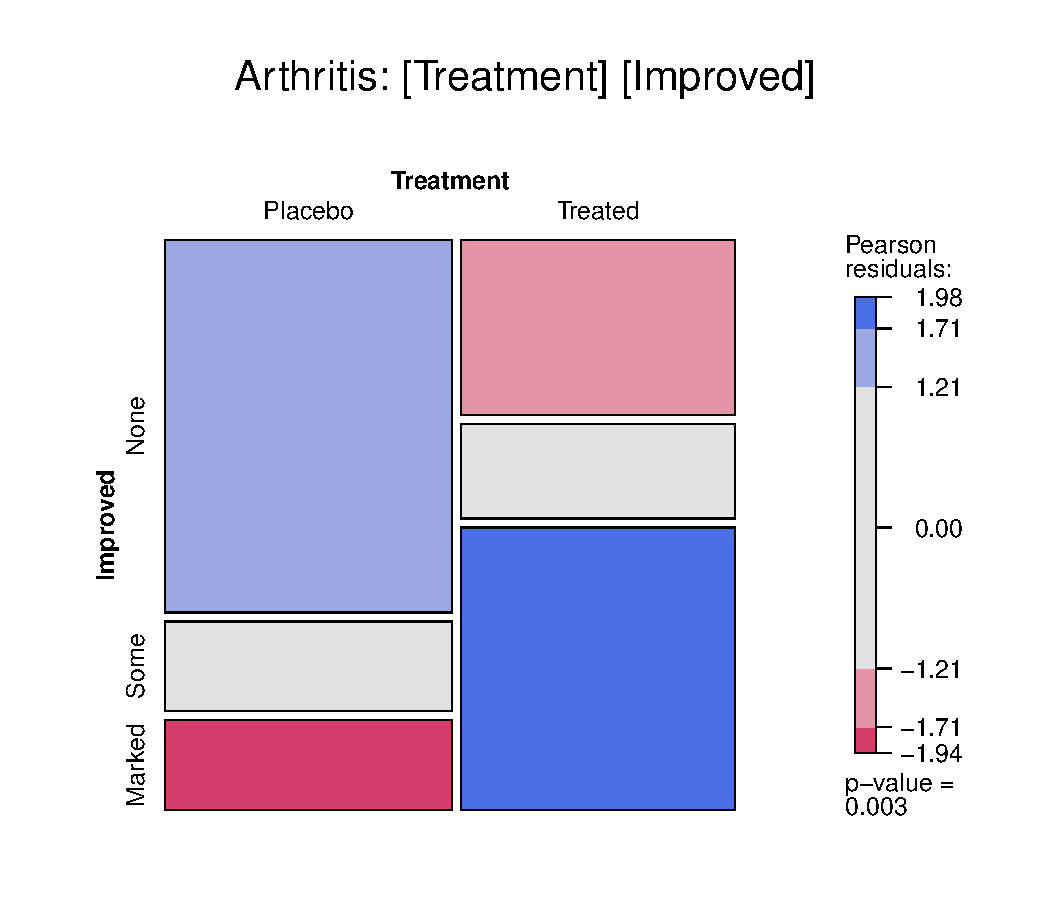
\includegraphics[width=0.7\textwidth]{fig/vcd-tut-Arthritis}
\caption{Mosaic plot for the \data{Arthritis} data, showing the marginal model of independence
	for Treatment and Improved.  Age, a covariate, and Sex are ignored here.}
\label{fig:arthritis}
\end{center}
\end{figure}

Finally, there are situations where, particularly for display purposes, you
want to re-order the \emph{dimensions} of an $n$-way table, or change the
labels for the variables or levels.
This is easy when the data are in table form: \codefun{aperm} permutes
the dimensions, and assigning to \code{names} and \code{dimnames}
changes variable names and level labels respectively.
We will use the following version of \data{UCBAdmissions} in
\secref{sec:mantel} below.%
\footnote{
Changing \code{Admit} to \code{Admit?} might be useful for display purposes, but is
dangerous--- because it is then
difficult to use that variable name in a model formula.
See \secref{sec:tips} for options \code{labeling\_args} and \code{set\_labels}
to change variable and level names 
for displays in the \code{strucplot} framework.
}
\begin{knitrout}
\definecolor{shadecolor}{rgb}{0.969, 0.969, 0.969}\color{fgcolor}\begin{kframe}
\begin{alltt}
\hlstd{UCB} \hlkwb{<-} \hlkwd{aperm}\hlstd{(UCBAdmissions,} \hlkwd{c}\hlstd{(}\hlnum{2}\hlstd{,} \hlnum{1}\hlstd{,} \hlnum{3}\hlstd{))}
\hlkwd{dimnames}\hlstd{(UCB)[[}\hlnum{2}\hlstd{]]} \hlkwb{<-} \hlkwd{c}\hlstd{(}\hlstr{"Yes"}\hlstd{,} \hlstr{"No"}\hlstd{)}
\hlkwd{names}\hlstd{(}\hlkwd{dimnames}\hlstd{(UCB))} \hlkwb{<-} \hlkwd{c}\hlstd{(}\hlstr{"Sex"}\hlstd{,} \hlstr{"Admit?"}\hlstd{,} \hlstr{"Department"}\hlstd{)}
\hlkwd{ftable}\hlstd{(UCB)}
\end{alltt}
\begin{verbatim}
##               Department   A   B   C   D   E   F
## Sex    Admit?                                   
## Male   Yes               512 353 120 138  53  22
##        No                313 207 205 279 138 351
## Female Yes                89  17 202 131  94  24
##        No                 19   8 391 244 299 317
\end{verbatim}
\end{kframe}
\end{knitrout}


\subsection[structable()]{\codefun{structable}}\label{sec:structable}
For 3-way and larger tables
the \codefun{structable} function in \pkg{vcd} provides a convenient and flexible tabular display.
The variables assigned to the rows and columns of a two-way display can be specified
by a model formula.
\begin{knitrout}
\definecolor{shadecolor}{rgb}{0.969, 0.969, 0.969}\color{fgcolor}\begin{kframe}
\begin{alltt}
\hlkwd{structable}\hlstd{(HairEyeColor)}                   \hlcom{# show the table: default}
\end{alltt}
\begin{verbatim}
##              Eye Brown Hazel Green Blue
## Hair  Sex                              
## Black Male          32    10     3   11
##       Female        36     5     2    9
## Brown Male          53    25    15   50
##       Female        66    29    14   34
## Red   Male          10     7     7   10
##       Female        16     7     7    7
## Blond Male           3     5     8   30
##       Female         4     5     8   64
\end{verbatim}
\begin{alltt}
\hlkwd{structable}\hlstd{(Hair}\hlopt{+}\hlstd{Sex} \hlopt{~} \hlstd{Eye, HairEyeColor)}   \hlcom{# specify col ~ row variables}
\end{alltt}
\begin{verbatim}
##       Hair Black        Brown         Red        Blond       
##       Sex   Male Female  Male Female Male Female  Male Female
## Eye                                                          
## Brown         32     36    53     66   10     16     3      4
## Hazel         10      5    25     29    7      7     5      5
## Green          3      2    15     14    7      7     8      8
## Blue          11      9    50     34   10      7    30     64
\end{verbatim}
\end{kframe}
\end{knitrout}

It also returns an object of class \code{"structable"} which may be plotted with 
\codefun{mosaic} (not shown here).
\begin{knitrout}
\definecolor{shadecolor}{rgb}{0.969, 0.969, 0.969}\color{fgcolor}\begin{kframe}
\begin{alltt}
\hlstd{HSE} \hlopt{< -} \hlkwd{structable}\hlstd{(Hair}\hlopt{+}\hlstd{Sex} \hlopt{~} \hlstd{Eye, HairEyeColor)}   \hlcom{# save structable object}
\hlkwd{mosaic}\hlstd{(HSE)}                                        \hlcom{# plot it}
\end{alltt}
\end{kframe}
\end{knitrout}


\subsection[table() and friends]{\codefun{table} and friends}\label{sec:table}

You  can  generate frequency  tables from factor variables  using the  \codefun{table} function,  tables  of
proportions using  the \codefun{prop.table} function,  and marginal  frequencies using
\codefun{margin.table}.

\begin{knitrout}
\definecolor{shadecolor}{rgb}{0.969, 0.969, 0.969}\color{fgcolor}\begin{kframe}
\begin{alltt}
 \hlstd{n}\hlkwb{=}\hlnum{500}
 \hlstd{A} \hlkwb{<-} \hlkwd{factor}\hlstd{(}\hlkwd{sample}\hlstd{(}\hlkwd{c}\hlstd{(}\hlstr{"a1"}\hlstd{,}\hlstr{"a2"}\hlstd{), n,} \hlkwc{rep}\hlstd{=}\hlnum{TRUE}\hlstd{))}
 \hlstd{B} \hlkwb{<-} \hlkwd{factor}\hlstd{(}\hlkwd{sample}\hlstd{(}\hlkwd{c}\hlstd{(}\hlstr{"b1"}\hlstd{,}\hlstr{"b2"}\hlstd{), n,} \hlkwc{rep}\hlstd{=}\hlnum{TRUE}\hlstd{))}
 \hlstd{C} \hlkwb{<-} \hlkwd{factor}\hlstd{(}\hlkwd{sample}\hlstd{(}\hlkwd{c}\hlstd{(}\hlstr{"c1"}\hlstd{,}\hlstr{"c2"}\hlstd{), n,} \hlkwc{rep}\hlstd{=}\hlnum{TRUE}\hlstd{))}
 \hlstd{mydata} \hlkwb{<-} \hlkwd{data.frame}\hlstd{(A,B,C)}
\end{alltt}
\end{kframe}
\end{knitrout}


\begin{knitrout}
\definecolor{shadecolor}{rgb}{0.969, 0.969, 0.969}\color{fgcolor}\begin{kframe}
\begin{alltt}
\hlcom{# 2-Way Frequency Table}
\hlkwd{attach}\hlstd{(mydata)}
\hlstd{mytable} \hlkwb{<-} \hlkwd{table}\hlstd{(A,B)}   \hlcom{# A will be rows, B will be columns}
\hlstd{mytable}                 \hlcom{# print table}
\hlkwd{margin.table}\hlstd{(mytable,} \hlnum{1}\hlstd{)} \hlcom{# A frequencies (summed over B)}
\hlkwd{margin.table}\hlstd{(mytable,} \hlnum{2}\hlstd{)} \hlcom{# B frequencies (summed over A)}
\hlkwd{prop.table}\hlstd{(mytable)}    \hlcom{# cell percentages}
\hlkwd{prop.table}\hlstd{(mytable,} \hlnum{1}\hlstd{)} \hlcom{# row percentages}
\hlkwd{prop.table}\hlstd{(mytable,} \hlnum{2}\hlstd{)} \hlcom{# column percentages}
\end{alltt}
\end{kframe}
\end{knitrout}


\codefun{table} can  also  generate  multidimensional  tables  based  on  3  or  more
categorical variables. In  this case, use  the \codefun{ftable}  or \codefun{structable}
function to print  the
results more attractively.

\begin{knitrout}
\definecolor{shadecolor}{rgb}{0.969, 0.969, 0.969}\color{fgcolor}\begin{kframe}
\begin{alltt}
\hlcom{# 3-Way Frequency Table}
\hlstd{mytable} \hlkwb{<-} \hlkwd{table}\hlstd{(A, B, C)}
\hlkwd{ftable}\hlstd{(mytable)}
\end{alltt}
\end{kframe}
\end{knitrout}


\codefun{table}  ignores missing values by default. 
To include \code{NA} as a category in counts, include the
table option  \code{exclude=NULL} if  the variable  is a  vector. If  the variable is a
factor you  have to  create a  new factor  using \code{newfactor  <- factor(oldfactor,
exclude=NULL)}. 

\subsection[xtabs()]{\codefun{xtabs}}\label{sec:xtabs}

The \codefun{xtabs} function allows you to create crosstabulations of data using formula style input.
This typically works with case-form data supplied in a data frame or a matrix.
The result is a contingency table in array format, whose dimensions are determined by  
the terms on the right side of the formula.

\begin{knitrout}
\definecolor{shadecolor}{rgb}{0.969, 0.969, 0.969}\color{fgcolor}\begin{kframe}
\begin{alltt}
\hlcom{# 3-Way Frequency Table}
\hlstd{mytable} \hlkwb{<-} \hlkwd{xtabs}\hlstd{(}\hlopt{~}\hlstd{A}\hlopt{+}\hlstd{B}\hlopt{+}\hlstd{C,} \hlkwc{data}\hlstd{=mydata)}
\hlkwd{ftable}\hlstd{(mytable)}    \hlcom{# print table}
\hlkwd{summary}\hlstd{(mytable)}   \hlcom{# chi-square test of indepedence}
\end{alltt}
\end{kframe}
\end{knitrout}


If a variable is included on the left side of the formula, it is assumed to be a
vector  of  frequencies  (useful if the data have already been tabulated in frequency form).

\begin{knitrout}
\definecolor{shadecolor}{rgb}{0.969, 0.969, 0.969}\color{fgcolor}\begin{kframe}
\begin{alltt}
\hlstd{(GSStab} \hlkwb{<-} \hlkwd{xtabs}\hlstd{(count} \hlopt{~} \hlstd{sex} \hlopt{+} \hlstd{party,} \hlkwc{data}\hlstd{=GSS))}
\end{alltt}
\begin{verbatim}
##         party
## sex      dem indep rep
##   female 279    73 225
##   male   165    47 191
\end{verbatim}
\begin{alltt}
\hlkwd{summary}\hlstd{(GSStab)}
\end{alltt}
\begin{verbatim}
## Call: xtabs(formula = count ~ sex + party, data = GSS)
## Number of cases in table: 980 
## Number of factors: 2 
## Test for independence of all factors:
## 	Chisq = 7, df = 2, p-value = 0.03
\end{verbatim}
\end{kframe}
\end{knitrout}


\subsection[Collapsing over factors]{Collapsing over table factors: \codefun{aggregate}, \codefun{margin.table} and \codefun{apply}}
It sometimes happens that we have a data set with more variables or factors than 
we want to analyse, or else, having done some initial analyses, we decide that
certain factors are not important, and so should be excluded from graphic displays
by collapsing (summing) over them.  For example, mosaic plots and fourfold displays
are often simpler to construct from versions of the data collapsed over
the factors which are not shown in the plots.

The appropriate tools to use again depend on
the form in which the data are represented--- a case-form data frame, a
frequency-form data frame (\codefun{aggregate}), or a table-form array or 
table object (\codefun{margin.table} or \codefun{apply}).

When the data are in frequency form, and we want to produce another
frequency data frame, \codefun{aggregate} is a handy tool, using
the argument \code{FUN=sum} to sum the frequency variable over the 
factors \emph{not} mentioned in the formula.

\Example 
The data frame \data{DaytonSurvey} in the \pkg{vcdExtra} package represents a
$2^5$ table giving the frequencies of reported use (``ever used?'') of 
alcohol, cigarettes and marijuana in a sample of high school seniors,
also classified by sex and race.  

\begin{knitrout}
\definecolor{shadecolor}{rgb}{0.969, 0.969, 0.969}\color{fgcolor}\begin{kframe}
\begin{alltt}
\hlkwd{str}\hlstd{(DaytonSurvey)}
\end{alltt}
\begin{verbatim}
## 'data.frame':	32 obs. of  6 variables:
##  $ cigarette: Factor w/ 2 levels "Yes","No": 1 2 1 2 1 2 1 2 1 2 ...
##  $ alcohol  : Factor w/ 2 levels "Yes","No": 1 1 2 2 1 1 2 2 1 1 ...
##  $ marijuana: Factor w/ 2 levels "Yes","No": 1 1 1 1 2 2 2 2 1 1 ...
##  $ sex      : Factor w/ 2 levels "female","male": 1 1 1 1 1 1 1 1 2 2 ...
##  $ race     : Factor w/ 2 levels "white","other": 1 1 1 1 1 1 1 1 1 1 ...
##  $ Freq     : num  405 13 1 1 268 218 17 117 453 28 ...
\end{verbatim}
\begin{alltt}
\hlkwd{head}\hlstd{(DaytonSurvey)}
\end{alltt}
\begin{verbatim}
##   cigarette alcohol marijuana    sex  race Freq
## 1       Yes     Yes       Yes female white  405
## 2        No     Yes       Yes female white   13
## 3       Yes      No       Yes female white    1
## 4        No      No       Yes female white    1
## 5       Yes     Yes        No female white  268
## 6        No     Yes        No female white  218
\end{verbatim}
\end{kframe}
\end{knitrout}


To focus on the associations among the
substances, we want to collapse over sex and race. The right-hand side of the formula
used in the call to \codefun{aggregate} gives the factors to be retained in the
new frequency data frame, \code{Dayton.ACM.df}.

\begin{knitrout}
\definecolor{shadecolor}{rgb}{0.969, 0.969, 0.969}\color{fgcolor}\begin{kframe}
\begin{alltt}
\hlcom{# data in frequency form}
\hlcom{# collapse over sex and race}
\hlstd{Dayton.ACM.df} \hlkwb{<-} \hlkwd{aggregate}\hlstd{(Freq} \hlopt{~} \hlstd{cigarette}\hlopt{+}\hlstd{alcohol}\hlopt{+}\hlstd{marijuana,}
                           \hlkwc{data}\hlstd{=DaytonSurvey,} \hlkwc{FUN}\hlstd{=sum)}
\hlstd{Dayton.ACM.df}
\end{alltt}
\begin{verbatim}
##   cigarette alcohol marijuana Freq
## 1       Yes     Yes       Yes  911
## 2        No     Yes       Yes   44
## 3       Yes      No       Yes    3
## 4        No      No       Yes    2
## 5       Yes     Yes        No  538
## 6        No     Yes        No  456
## 7       Yes      No        No   43
## 8        No      No        No  279
\end{verbatim}
\end{kframe}
\end{knitrout}


When the data are in table form, and we want to produce another
table, \codefun{apply} with \code{FUN=sum} can be used in a similar way
to sum the table over dimensions not mentioned in the \code{MARGIN}
argument.  \codefun{margin.table} is just a wrapper for \codefun{apply}
using the \codefun{sum} function.


\Example 
To illustrate, we first convert the \data{DaytonSurvey} to a 5-way
table using \codefun{xtabs}, giving \code{Dayton.tab}.  

\begin{knitrout}
\definecolor{shadecolor}{rgb}{0.969, 0.969, 0.969}\color{fgcolor}\begin{kframe}
\begin{alltt}
\hlcom{# in table form}
\hlstd{Dayton.tab} \hlkwb{<-} \hlkwd{xtabs}\hlstd{(Freq}\hlopt{~}\hlstd{cigarette}\hlopt{+}\hlstd{alcohol}\hlopt{+}\hlstd{marijuana}\hlopt{+}\hlstd{sex}\hlopt{+}\hlstd{race,} \hlkwc{data}\hlstd{=DaytonSurvey)}
\hlkwd{structable}\hlstd{(cigarette}\hlopt{+}\hlstd{alcohol}\hlopt{+}\hlstd{marijuana} \hlopt{~} \hlstd{sex}\hlopt{+}\hlstd{race,} \hlkwc{data}\hlstd{=Dayton.tab)}
\end{alltt}
\begin{verbatim}
##              cigarette Yes              No            
##              alcohol   Yes      No     Yes      No    
##              marijuana Yes  No Yes  No Yes  No Yes  No
## sex    race                                           
## female white           405 268   1  17  13 218   1 117
##        other            23  23   0   1   2  19   0  12
## male   white           453 228   1  17  28 201   1 133
##        other            30  19   1   8   1  18   0  17
\end{verbatim}
\end{kframe}
\end{knitrout}

Then, use \codefun{apply} on \code{Dayton.tab} to give the
3-way table \code{Dayton.ACM.tab} summed over sex and race.
The elements in this new table are the column sums for 
\code{Dayton.tab} shown by \codefun{structable} just above.

\begin{knitrout}
\definecolor{shadecolor}{rgb}{0.969, 0.969, 0.969}\color{fgcolor}\begin{kframe}
\begin{alltt}
\hlcom{# collapse over sex and race}
\hlstd{Dayton.ACM.tab} \hlkwb{<-} \hlkwd{apply}\hlstd{(Dayton.tab,} \hlkwc{MARGIN}\hlstd{=}\hlnum{1}\hlopt{:}\hlnum{3}\hlstd{,} \hlkwc{FUN}\hlstd{=sum)}
\hlstd{Dayton.ACM.tab} \hlkwb{<-} \hlkwd{margin.table}\hlstd{(Dayton.tab,} \hlnum{1}\hlopt{:}\hlnum{3}\hlstd{)}   \hlcom{# same result}
\hlkwd{structable}\hlstd{(cigarette}\hlopt{+}\hlstd{alcohol} \hlopt{~} \hlstd{marijuana,} \hlkwc{data}\hlstd{=Dayton.ACM.tab)}
\end{alltt}
\begin{verbatim}
##           cigarette Yes      No    
##           alcohol   Yes  No Yes  No
## marijuana                          
## Yes                 911   3  44   2
## No                  538  43 456 279
\end{verbatim}
\end{kframe}
\end{knitrout}




Many of these operations can be performed using the \verb|**ply()| functions
in the \pkg{plyr} package.
For example, with the data in a frequency form data frame, use \codefun{ddply}
to collapse over unmentioned factors, and \codefun{plyr::summarise}%
\footnote{
Ugh. This \pkg{plyr} function clashes with a function of the same name in \pkg{vcdExtra}.
In this document I will use the explicit double-colon notation to keep them
separate.
}
as the function to be applied to each piece.
\begin{knitrout}
\definecolor{shadecolor}{rgb}{0.969, 0.969, 0.969}\color{fgcolor}\begin{kframe}
\begin{alltt}
\hlstd{Dayton.ACM.df} \hlkwb{<-} \hlkwd{ddply}\hlstd{(DaytonSurvey,} \hlkwd{.}\hlstd{(cigarette, alcohol, marijuana),}
                       \hlstd{plyr::summarise,} \hlkwc{Freq}\hlstd{=}\hlkwd{sum}\hlstd{(Freq))}
\end{alltt}
\end{kframe}
\end{knitrout}


\subsection[Collapsing levels]{Collapsing table levels: \codefun{collapse.table}}

A related problem arises when we have a table or array and for some purpose
we want to reduce the number of levels of some factors by summing subsets
of the frequencies.  For example, we may have initially coded Age in 10-year
intervals, and decide that, either for analysis or display purposes, we
want to reduce Age to 20-year intervals.  The \codefun{collapse.table} function
in \pkg{vcdExtra} was designed for this purpose.

\Example
Create a 3-way table, and collapse Age from 10-year to 20-year intervals. 
First, we generate a $2 \times 6 \times 3$ table of random counts from a 
Poisson distribution with mean of 100.
\begin{knitrout}
\definecolor{shadecolor}{rgb}{0.969, 0.969, 0.969}\color{fgcolor}\begin{kframe}
\begin{alltt}
\hlcom{# create some sample data in frequency form}
\hlstd{sex} \hlkwb{<-} \hlkwd{c}\hlstd{(}\hlstr{"Male"}\hlstd{,} \hlstr{"Female"}\hlstd{)}
\hlstd{age} \hlkwb{<-} \hlkwd{c}\hlstd{(}\hlstr{"10-19"}\hlstd{,} \hlstr{"20-29"}\hlstd{,}  \hlstr{"30-39"}\hlstd{,} \hlstr{"40-49"}\hlstd{,} \hlstr{"50-59"}\hlstd{,} \hlstr{"60-69"}\hlstd{)}
\hlstd{education} \hlkwb{<-} \hlkwd{c}\hlstd{(}\hlstr{"low"}\hlstd{,} \hlstr{'med'}\hlstd{,} \hlstr{'high'}\hlstd{)}
\hlstd{data} \hlkwb{<-} \hlkwd{expand.grid}\hlstd{(}\hlkwc{sex}\hlstd{=sex,} \hlkwc{age}\hlstd{=age,} \hlkwc{education}\hlstd{=education)}
\hlstd{counts} \hlkwb{<-} \hlkwd{rpois}\hlstd{(}\hlnum{36}\hlstd{,} \hlnum{100}\hlstd{)}   \hlcom{# random Possion cell frequencies}
\hlstd{data} \hlkwb{<-} \hlkwd{cbind}\hlstd{(data, counts)}
\hlcom{# make it into a 3-way table}
\hlstd{t1} \hlkwb{<-} \hlkwd{xtabs}\hlstd{(counts} \hlopt{~} \hlstd{sex} \hlopt{+} \hlstd{age} \hlopt{+} \hlstd{education,} \hlkwc{data}\hlstd{=data)}
\hlkwd{structable}\hlstd{(t1)}
\end{alltt}
\begin{verbatim}
##                  age 10-19 20-29 30-39 40-49 50-59 60-69
## sex    education                                        
## Male   low              98   105   104    90    90   101
##        med              97   105   101    88    97   107
##        high             99   101   109    88    99    96
## Female low             102   117   101   105    85    88
##        med             106    84    92   116   110    96
##        high            106    96   121    91   107   102
\end{verbatim}
\end{kframe}
\end{knitrout}

Now collapse \code{age} to 20-year intervals, and \code{education}
to 2 levels. In the arguments, levels of \code{age} and \code{education}
given the same label are summed in the resulting smaller table.
\begin{knitrout}
\definecolor{shadecolor}{rgb}{0.969, 0.969, 0.969}\color{fgcolor}\begin{kframe}
\begin{alltt}
\hlcom{# collapse age to 3 levels, education to 2 levels}
\hlstd{t2} \hlkwb{<-} \hlkwd{collapse.table}\hlstd{(t1,}
         \hlkwc{age}\hlstd{=}\hlkwd{c}\hlstd{(}\hlstr{"10-29"}\hlstd{,} \hlstr{"10-29"}\hlstd{,}  \hlstr{"30-49"}\hlstd{,} \hlstr{"30-49"}\hlstd{,} \hlstr{"50-69"}\hlstd{,} \hlstr{"50-69"}\hlstd{),}
         \hlkwc{education}\hlstd{=}\hlkwd{c}\hlstd{(}\hlstr{"<high"}\hlstd{,} \hlstr{"<high"}\hlstd{,} \hlstr{"high"}\hlstd{))}
\hlkwd{structable}\hlstd{(t2)}
\end{alltt}
\begin{verbatim}
##                  age 10-29 30-49 50-69
## sex    education                      
## Male   <high           405   383   395
##        high            200   197   195
## Female <high           409   414   379
##        high            202   212   209
\end{verbatim}
\end{kframe}
\end{knitrout}



\subsection[Converting]{Converting among frequency tables and data frames}

As we've seen, a given contingency table can be represented 
equivalently in different forms,
but some \proglang{R} functions were designed for one particular representation.
\tabref{tab:convert} shows some handy tools for converting from one form to another.

\begin{table}[htb]
 \caption{Tools for converting among different forms for categorical data}\label{tab:convert}
 \begin{center}
   \begin{tabular}{llll}
	\hline
                 & \multicolumn{3}{c}{\textbf{To this}} \\
	\textbf{From this}      &     Case form         & Frequency form             &  Table form \\
	\hline
	Case form      &   noop                 & \verb|xtabs(~A+B)|        &  \verb|table(A,B)|  \\ 
	Frequency form &  \verb|expand.dft(X)|  & noop                      & \verb|xtabs(count~A+B)|\\
	Table form     &  \verb|expand.dft(X)|  & \verb|as.data.frame(X)|   &  noop \\
	\hline
   \end{tabular}
 \end{center}
\end{table}

A contingency table in table form (an object of \code{class(table)}) can be converted
to a data.frame with \codefun{as.data.frame}.%
\footnote{
Because \proglang{R} is object-oriented, this is actually a short-hand for
the function \codefun{as.data.frame.table}.
}  
The resulting
\code{data.frame} contains columns
representing the classifying factors and the table entries (as a column named by
the \code{responseName} argument, defaulting to \code{Freq}. This is the inverse of \codefun{xtabs}.

\Example 
Convert the \code{GSStab} in table form to a data.frame in frequency form.
\begin{knitrout}
\definecolor{shadecolor}{rgb}{0.969, 0.969, 0.969}\color{fgcolor}\begin{kframe}
\begin{alltt}
\hlkwd{as.data.frame}\hlstd{(GSStab)}
\end{alltt}
\begin{verbatim}
##      sex party Freq
## 1 female   dem  279
## 2   male   dem  165
## 3 female indep   73
## 4   male indep   47
## 5 female   rep  225
## 6   male   rep  191
\end{verbatim}
\end{kframe}
\end{knitrout}


\Example Convert the \code{Arthritis} data in case form to a 3-way table of
\code{Treatment} $\times$ \code{Sex} $\times$ \code{Improved}.
Note the use of \codefun{with} to avoid having to use \code{Arthritis\$Treatment} etc. within the call to \codefun{table}.%
\footnote{
\codefun{table} does not allow a \code{data} argument to provide
an environment in which the table variables are to be found.  In the 
examples in \secref{sec:table} I used \code{attach(mydata)} for this purpose,
but \codefun{attach} leaves the variables in the global environment,
while \codefun{with} just evaluates the \codefun{table} expression in a
temporary environment of the data.
}
\begin{knitrout}
\definecolor{shadecolor}{rgb}{0.969, 0.969, 0.969}\color{fgcolor}\begin{kframe}
\begin{alltt}
\hlstd{Art.tab} \hlkwb{<-}\hlkwd{with}\hlstd{(Arthritis,} \hlkwd{table}\hlstd{(Treatment, Sex, Improved))}
\hlkwd{str}\hlstd{(Art.tab)}
\end{alltt}
\begin{verbatim}
##  'table' int [1:2, 1:2, 1:3] 19 6 10 7 7 5 0 2 6 16 ...
##  - attr(*, "dimnames")=List of 3
##   ..$ Treatment: chr [1:2] "Placebo" "Treated"
##   ..$ Sex      : chr [1:2] "Female" "Male"
##   ..$ Improved : chr [1:3] "None" "Some" "Marked"
\end{verbatim}
\begin{alltt}
\hlkwd{ftable}\hlstd{(Art.tab)}
\end{alltt}
\begin{verbatim}
##                  Improved None Some Marked
## Treatment Sex                             
## Placebo   Female            19    7      6
##           Male              10    0      1
## Treated   Female             6    5     16
##           Male               7    2      5
\end{verbatim}
\end{kframe}
\end{knitrout}



There may also be times that you will need an equivalent case form \code{data.frame}
with factors  representing the table variables
rather than the frequency  table.
For example, the \codefun{mca} function in package \pkg{MASS}
only operates on data in this format. 
Marc Schwartz provided code for \codefun{expand.dft} on the  Rhelp
mailing list for converting a table back into a case form \code{data.frame}.
This function is included in \pkg{vcdExtra}.

\Example Convert the \data{Arthritis} data in table form (\code{Art.tab}) back to a \code{data.frame}
in case form, with factors
\code{Treatment}, \code{Sex} and \code{Improved}.
\begin{knitrout}
\definecolor{shadecolor}{rgb}{0.969, 0.969, 0.969}\color{fgcolor}\begin{kframe}
\begin{alltt}
\hlstd{Art.df} \hlkwb{<-} \hlkwd{expand.dft}\hlstd{(Art.tab)}
\hlkwd{str}\hlstd{(Art.df)}
\end{alltt}
\begin{verbatim}
## 'data.frame':	84 obs. of  3 variables:
##  $ Treatment: Factor w/ 2 levels "Placebo","Treated": 1 1 1 1 1 1 1 1 1 1 ...
##  $ Sex      : Factor w/ 2 levels "Female","Male": 1 1 1 1 1 1 1 1 1 1 ...
##  $ Improved : Factor w/ 3 levels "Marked","None",..: 2 2 2 2 2 2 2 2 2 2 ...
\end{verbatim}
\end{kframe}
\end{knitrout}


\subsection{A complex example}\label{sec:complex}

If you've followed so far, you're ready for a more complicated example.
The data file, \code{tv.dat} represents a 4-way table of size
$5 \times 11 \times 5 \times 3$ where the table variables (unnamed in the file)
are read as \code{V1} -- \code{V4}, and the cell frequency is read
as \code{V5}.  The file, stored in the \code{doc/extdata} directory
of \pkg{vcdExtra}, can be read as follows:
\begin{knitrout}
\definecolor{shadecolor}{rgb}{0.969, 0.969, 0.969}\color{fgcolor}\begin{kframe}
\begin{alltt}
\hlstd{tv.data}\hlkwb{<-}\hlkwd{read.table}\hlstd{(}\hlkwd{system.file}\hlstd{(}\hlstr{"doc"}\hlstd{,}\hlstr{"extdata"}\hlstd{,}\hlstr{"tv.dat"}\hlstd{,}\hlkwc{package}\hlstd{=}\hlstr{"vcdExtra"}\hlstd{))}
\hlkwd{head}\hlstd{(tv.data,}\hlnum{5}\hlstd{)}
\end{alltt}
\begin{verbatim}
##   V1 V2 V3 V4 V5
## 1  1  1  1  1  6
## 2  2  1  1  1 18
## 3  3  1  1  1  6
## 4  4  1  1  1  2
## 5  5  1  1  1 11
\end{verbatim}
\end{kframe}
\end{knitrout}

For a local file, just use \codefun{read.table} in this form:
\begin{knitrout}
\definecolor{shadecolor}{rgb}{0.969, 0.969, 0.969}\color{fgcolor}\begin{kframe}
\begin{alltt}
\hlstd{tv.data}\hlkwb{<-}\hlkwd{read.table}\hlstd{(}\hlstr{"C:/R/data/tv.dat"}\hlstd{)}
\end{alltt}
\end{kframe}
\end{knitrout}

The data \code{tv.dat} came from the initial implementation of 
mosaic displays in \proglang{R} by Jay Emerson. 
In turn, they came from the initial development of mosaic displays 
\citep{vcd:Hartigan+Kleiner:1984}
that illustrated the method with data on a large sample of TV viewers
whose behavior had been recorded for the Neilson ratings.
This data set contains sample television audience data from Neilsen
Media Research for the week starting November 6, 1995.

\begin{flushleft}
The table variables are:\\
~~~\code{V1}-- values 1:5 correspond to the days Monday--Friday;\\
~~~\code{V2}-- values 1:11 correspond to the quarter hour times 8:00PM through 10:30PM;\\
~~~\code{V3}-- values 1:5 correspond to ABC, CBS, NBC, Fox, and non-network choices;\\
~~~\code{V4}-- values 1:3 correspond to transition states: turn the television Off, Switch channels, 
 or Persist in viewing the current channel.
\end{flushleft}
	 
We are interested just the cell frequencies, and rely on the facts that the
(a) the table is complete--- there are no missing cells,
so \code{nrow(tv.data)}=825;
(b) the observations are ordered so that \code{V1} varies most rapidly and
\code{V4} most slowly.  From this, we can just extract the frequency column
and reshape it into an array.
\begin{knitrout}
\definecolor{shadecolor}{rgb}{0.969, 0.969, 0.969}\color{fgcolor}\begin{kframe}
\begin{alltt}
\hlstd{TV} \hlkwb{<-} \hlkwd{array}\hlstd{(tv.data[,}\hlnum{5}\hlstd{],} \hlkwc{dim}\hlstd{=}\hlkwd{c}\hlstd{(}\hlnum{5}\hlstd{,}\hlnum{11}\hlstd{,}\hlnum{5}\hlstd{,}\hlnum{3}\hlstd{))}
\hlkwd{dimnames}\hlstd{(TV)} \hlkwb{<-} \hlkwd{list}\hlstd{(}\hlkwd{c}\hlstd{(}\hlstr{"Monday"}\hlstd{,}\hlstr{"Tuesday"}\hlstd{,}\hlstr{"Wednesday"}\hlstd{,}\hlstr{"Thursday"}\hlstd{,}\hlstr{"Friday"}\hlstd{),}
                \hlkwd{c}\hlstd{(}\hlstr{"8:00"}\hlstd{,}\hlstr{"8:15"}\hlstd{,}\hlstr{"8:30"}\hlstd{,}\hlstr{"8:45"}\hlstd{,}\hlstr{"9:00"}\hlstd{,}\hlstr{"9:15"}\hlstd{,}\hlstr{"9:30"}\hlstd{,}
                  \hlstr{"9:45"}\hlstd{,}\hlstr{"10:00"}\hlstd{,}\hlstr{"10:15"}\hlstd{,}\hlstr{"10:30"}\hlstd{),}
                \hlkwd{c}\hlstd{(}\hlstr{"ABC"}\hlstd{,}\hlstr{"CBS"}\hlstd{,}\hlstr{"NBC"}\hlstd{,}\hlstr{"Fox"}\hlstd{,}\hlstr{"Other"}\hlstd{),} \hlkwd{c}\hlstd{(}\hlstr{"Off"}\hlstd{,}\hlstr{"Switch"}\hlstd{,}\hlstr{"Persist"}\hlstd{))}
\hlkwd{names}\hlstd{(}\hlkwd{dimnames}\hlstd{(TV))}\hlkwb{<-}\hlkwd{c}\hlstd{(}\hlstr{"Day"}\hlstd{,} \hlstr{"Time"}\hlstd{,} \hlstr{"Network"}\hlstd{,} \hlstr{"State"}\hlstd{)}
\end{alltt}
\end{kframe}
\end{knitrout}


More generally (even if there are missing cells), we can 
use \codefun{xtabs} (or \codefun{plyr::daply})
to do the cross-tabulation, using \code{V5} as the
frequency variable.  Here's how to do this same operation with \codefun{xtabs}:
\begin{knitrout}
\definecolor{shadecolor}{rgb}{0.969, 0.969, 0.969}\color{fgcolor}\begin{kframe}
\begin{alltt}
\hlstd{TV} \hlkwb{<-} \hlkwd{xtabs}\hlstd{(V5} \hlopt{~} \hlstd{.,} \hlkwc{data}\hlstd{=tv.data)}
\hlkwd{dimnames}\hlstd{(TV)} \hlkwb{<-} \hlkwd{list}\hlstd{(}\hlkwc{Day}\hlstd{=}\hlkwd{c}\hlstd{(}\hlstr{"Monday"}\hlstd{,}\hlstr{"Tuesday"}\hlstd{,}\hlstr{"Wednesday"}\hlstd{,}\hlstr{"Thursday"}\hlstd{,}\hlstr{"Friday"}\hlstd{),}
                \hlkwc{Time}\hlstd{=}\hlkwd{c}\hlstd{(}\hlstr{"8:00"}\hlstd{,}\hlstr{"8:15"}\hlstd{,}\hlstr{"8:30"}\hlstd{,}\hlstr{"8:45"}\hlstd{,}\hlstr{"9:00"}\hlstd{,}\hlstr{"9:15"}\hlstd{,}\hlstr{"9:30"}\hlstd{,}
                       \hlstr{"9:45"}\hlstd{,}\hlstr{"10:00"}\hlstd{,}\hlstr{"10:15"}\hlstd{,}\hlstr{"10:30"}\hlstd{),}
                \hlkwc{Network}\hlstd{=}\hlkwd{c}\hlstd{(}\hlstr{"ABC"}\hlstd{,}\hlstr{"CBS"}\hlstd{,}\hlstr{"NBC"}\hlstd{,}\hlstr{"Fox"}\hlstd{,}\hlstr{"Other"}\hlstd{),}
                \hlkwc{State}\hlstd{=}\hlkwd{c}\hlstd{(}\hlstr{"Off"}\hlstd{,}\hlstr{"Switch"}\hlstd{,}\hlstr{"Persist"}\hlstd{))}
\end{alltt}
\end{kframe}
\end{knitrout}


But this 4-way table is too large and awkward to work with. Among the networks,
Fox and Other occur infrequently. 
We can also cut it down to a 3-way table by considering only viewers who persist
with the current station.%
\footnote{This relies on the fact that that indexing
an array drops dimensions of length 1 by default,
using the argument \code{drop=TRUE};
the result is coerced to the lowest possible dimension.
}

\begin{knitrout}
\definecolor{shadecolor}{rgb}{0.969, 0.969, 0.969}\color{fgcolor}\begin{kframe}
\begin{alltt}
\hlstd{TV} \hlkwb{<-} \hlstd{TV[,,}\hlnum{1}\hlopt{:}\hlnum{3}\hlstd{,]}     \hlcom{# keep only ABC, CBS, NBC}
\hlstd{TV} \hlkwb{<-} \hlstd{TV[,,,}\hlnum{3}\hlstd{]}       \hlcom{# keep only Persist -- now a 3 way table}
\hlkwd{structable}\hlstd{(TV)}
\end{alltt}
\begin{verbatim}
##                   Time 8:00 8:15 8:30 8:45 9:00 9:15 9:30 9:45 10:00 10:15 10:30
## Day       Network                                                               
## Monday    ABC           146  151  156   83  325  350  386  340   352   280   278
##           CBS           337  293  304  233  311  251  241  164   252   265   272
##           NBC           263  219  236  140  226  235  239  246   279   263   283
## Tuesday   ABC           244  181  231  205  385  283  345  192   329   351   364
##           CBS           173  180  184  109  218  235  256  250   274   263   261
##           NBC           315  254  280  241  370  214  195  111   188   190   210
## Wednesday ABC           233  161  194  156  339  264  279  140   237   228   203
##           CBS           158  126  207   59   98  103  122   86   109   105   110
##           NBC           134  146  166   66  194  230  264  143   274   289   306
## Thursday  ABC           174  183  197  181  187  198  211   86   110   122   117
##           CBS           196  185  195  104  106  116  116   47   102    84    84
##           NBC           515  463  472  477  590  473  446  349   649   705   747
## Friday    ABC           294  281  305  239  278  246  245  138   246   232   233
##           CBS           130  144  154   81  129  153  136  126   138   136   152
##           NBC           195  220  248  160  172  164  169   85   183   198   204
\end{verbatim}
\end{kframe}
\end{knitrout}


Finally, for some purposes, we might want to collapse the 11 times into a smaller number.
Here, we use \codefun{as.data.frame.table} to convert the table back to a data frame,
 \codefun{levels} to re-assign the values of \code{Time},
 and finally, \codefun{xtabs} to give a new, collapsed frequency table.

\begin{knitrout}
\definecolor{shadecolor}{rgb}{0.969, 0.969, 0.969}\color{fgcolor}\begin{kframe}
\begin{alltt}
\hlstd{TV.df} \hlkwb{<-} \hlkwd{as.data.frame.table}\hlstd{(TV)}
\hlkwd{levels}\hlstd{(TV.df}\hlopt{$}\hlstd{Time)} \hlkwb{<-} \hlkwd{c}\hlstd{(}\hlkwd{rep}\hlstd{(}\hlstr{"8:00-8:59"}\hlstd{,}\hlnum{4}\hlstd{),}\hlkwd{rep}\hlstd{(}\hlstr{"9:00-9:59"}\hlstd{,}\hlnum{4}\hlstd{),} \hlkwd{rep}\hlstd{(}\hlstr{"10:00-10:44"}\hlstd{,}\hlnum{3}\hlstd{))}
\hlstd{TV2} \hlkwb{<-} \hlkwd{xtabs}\hlstd{(Freq} \hlopt{~} \hlstd{Day} \hlopt{+} \hlstd{Time} \hlopt{+} \hlstd{Network, TV.df)}
\hlkwd{structable}\hlstd{(Day} \hlopt{~} \hlstd{Time}\hlopt{+}\hlstd{Network,TV2)}
\end{alltt}
\begin{verbatim}
##                     Day Monday Tuesday Wednesday Thursday Friday
## Time        Network                                             
## 8:00-8:59   ABC            536     861       744      735   1119
##             CBS           1167     646       550      680    509
##             NBC            858    1090       512     1927    823
## 9:00-9:59   ABC           1401    1205      1022      682    907
##             CBS            967     959       409      385    544
##             NBC            946     890       831     1858    590
## 10:00-10:44 ABC            910    1044       668      349    711
##             CBS            789     798       324      270    426
##             NBC            825     588       869     2101    585
\end{verbatim}
\end{kframe}
\end{knitrout}

Whew! See \figref{fig:TV-mosaic} for a mosaic plot of the \code{TV2} data.


\section{Tests of Independence}

\subsection{CrossTable}

OK, now we're ready to do some analyses.  For tabular displays,
the  \codefun{CrossTable}  function in  the \pkg{gmodels}  package produces  cross-tabulations
modeled after \code{PROC FREQ} in \proglang{SAS} or \code{CROSSTABS} in \proglang{SPSS}. 
It has a wealth of options for the quantities that can be shown in each cell.

\begin{knitrout}
\definecolor{shadecolor}{rgb}{0.969, 0.969, 0.969}\color{fgcolor}\begin{kframe}
\begin{alltt}
\hlcom{# 2-Way Cross Tabulation}
\hlkwd{library}\hlstd{(gmodels)}
\hlkwd{CrossTable}\hlstd{(GSStab,}\hlkwc{prop.t}\hlstd{=}\hlnum{FALSE}\hlstd{,}\hlkwc{prop.r}\hlstd{=}\hlnum{FALSE}\hlstd{,}\hlkwc{prop.c}\hlstd{=}\hlnum{FALSE}\hlstd{)}
\end{alltt}
\begin{verbatim}
## 
##  
##    Cell Contents
## |-------------------------|
## |                       N |
## | Chi-square contribution |
## |-------------------------|
## 
##  
## Total Observations in Table:  980 
## 
##  
##              | party 
##          sex |       dem |     indep |       rep | Row Total | 
## -------------|-----------|-----------|-----------|-----------|
##       female |       279 |        73 |       225 |       577 | 
##              |     1.183 |     0.078 |     1.622 |           | 
## -------------|-----------|-----------|-----------|-----------|
##         male |       165 |        47 |       191 |       403 | 
##              |     1.693 |     0.112 |     2.322 |           | 
## -------------|-----------|-----------|-----------|-----------|
## Column Total |       444 |       120 |       416 |       980 | 
## -------------|-----------|-----------|-----------|-----------|
## 
## 
\end{verbatim}
\end{kframe}
\end{knitrout}

There are  options to  report percentages  (row, column,  cell), specify decimal
places, produce Chi-square,  Fisher, and McNemar  tests of independence,  report
expected  and residual  values (pearson,  standardized, adjusted  standardized),
include missing values as valid, annotate with row and column titles, and format
as \proglang{SAS} or \proglang{SPSS} style output! See \code{help(CrossTable)} for details.


\subsection{Chi-square test}

For 2-way tables you can use \codefun{chisq.test} to test independence of the row
and column variable. By default,  the $p$-value is calculated from  the asymptotic
chi-squared distribution of the test  statistic. Optionally, the $p$-value can  be
derived via Monte Carlo simulation. 

\begin{knitrout}
\definecolor{shadecolor}{rgb}{0.969, 0.969, 0.969}\color{fgcolor}\begin{kframe}
\begin{alltt}
\hlstd{(HairEye} \hlkwb{<-} \hlkwd{margin.table}\hlstd{(HairEyeColor,} \hlkwd{c}\hlstd{(}\hlnum{1}\hlstd{,} \hlnum{2}\hlstd{)))}
\end{alltt}
\begin{verbatim}
##        Eye
## Hair    Brown Hazel Green Blue
##   Black    68    15     5   20
##   Brown   119    54    29   84
##   Red      26    14    14   17
##   Blond     7    10    16   94
\end{verbatim}
\begin{alltt}
\hlkwd{chisq.test}\hlstd{(HairEye)}
\end{alltt}
\begin{verbatim}
## 
## 	Pearson's Chi-squared test
## 
## data:  HairEye
## X-squared = 138.3, df = 9, p-value < 2.2e-16
\end{verbatim}
\end{kframe}
\end{knitrout}


\subsection{Fisher Exact Test}\label{sec:Fisher}

\code{fisher.test(X)} provides an  exact test of  independence. \code{X} must be  a two-way
contingency table in table form.  Another form, 
\code{fisher.test(X, Y)} takes two
categorical vectors of the same length.  
For tables larger than $2 \times 2$ the method can be computationally intensive (or can fail) if
the frequencies are not small.

\begin{knitrout}
\definecolor{shadecolor}{rgb}{0.969, 0.969, 0.969}\color{fgcolor}\begin{kframe}
\begin{alltt}
\hlkwd{fisher.test}\hlstd{(GSStab)}
\end{alltt}
\begin{verbatim}
## 
## 	Fisher's Exact Test for Count Data
## 
## data:  GSStab
## p-value = 0.03115
## alternative hypothesis: two.sided
\end{verbatim}
\end{kframe}
\end{knitrout}


But this does not work because \data{HairEye} data has $n$=592 total frequency.
An exact test is unnecessary in this case.
\begin{knitrout}
\definecolor{shadecolor}{rgb}{0.969, 0.969, 0.969}\color{fgcolor}\begin{kframe}
\begin{alltt}
\hlkwd{fisher.test}\hlstd{(HairEye)}
\end{alltt}
\end{kframe}
\end{knitrout}

%# <<echo=TRUE,eval=FALSE,results='markup'>>=
%# #cat(try(fisher.test(HairEye)))
%# @
\begin{verbatim}
## Error in fisher.test(HairEye) : FEXACT error 6.
## LDKEY is too small for this problem.
## Try increasing the size of the workspace.
\end{verbatim}

\subsection[Mantel-Haenszel test]{Mantel-Haenszel test and conditional association}\label{sec:mantel}

Use the  \code{mantelhaen.test(X)} function  to perform  a Cochran-Mantel-Haenszel 
$\chi^2$ chi
test  of   the  null  hypothesis   that  two  nominal   variables  are
\emph{conditionally independent}, $A \perp B \given C$, in each stratum,  assuming that there is no  three-way
interaction. \code{X} is  a 3 dimensional  contingency table, where  the last dimension
refers to the strata.

The \data{UCBAdmissions} serves as an example of a $2 \times 2 \times 6$ table,
with \code{Dept} as the stratifying variable.
\begin{knitrout}
\definecolor{shadecolor}{rgb}{0.969, 0.969, 0.969}\color{fgcolor}\begin{kframe}
\begin{alltt}
\hlcom{## UC Berkeley Student Admissions}
\hlkwd{mantelhaen.test}\hlstd{(UCBAdmissions)}
\end{alltt}
\begin{verbatim}
## 
## 	Mantel-Haenszel chi-squared test with continuity correction
## 
## data:  UCBAdmissions
## Mantel-Haenszel X-squared = 1.427, df = 1, p-value = 0.2323
## alternative hypothesis: true common odds ratio is not equal to 1
## 95 percent confidence interval:
##  0.7719 1.0603
## sample estimates:
## common odds ratio 
##            0.9047
\end{verbatim}
\end{kframe}
\end{knitrout}

The results show no evidence for association between admission and gender
when adjusted for department.  However, we can easily see that the assumption
of equal association across the strata (no 3-way association) is probably
violated. For $2 \times 2 \times k$ tables, this can be examimed
from the odds ratios for each $2 \times 2$ table (\codefun{oddsratio}), and
tested 
by  using
\verb|woolf_test()| in \pkg{vcd}.

%<<mantel2,results='markup'>>=
%oddsRatio <- function(x) (x[1,1]*x[2,2])/(x[1,2]*x[2,1])
%apply(UCBAdmissions, 3, oddsRatio)
%
%woolf_test(UCBAdmissions) 
%@ 
\begin{knitrout}
\definecolor{shadecolor}{rgb}{0.969, 0.969, 0.969}\color{fgcolor}\begin{kframe}
\begin{alltt}
\hlkwd{oddsratio}\hlstd{(UCBAdmissions,} \hlkwc{log}\hlstd{=}\hlnum{FALSE}\hlstd{)}
\end{alltt}
\begin{verbatim}
##      A      B      C      D      E      F 
## 0.3492 0.8025 1.1331 0.9213 1.2216 0.8279
\end{verbatim}
\begin{alltt}
\hlstd{lor} \hlkwb{<-} \hlkwd{oddsratio}\hlstd{(UCBAdmissions)}  \hlcom{# capture log odds ratios}
\hlkwd{summary}\hlstd{(lor)}
\end{alltt}
\begin{verbatim}
##   Log Odds Ratio Std. Error z value Pr(>|z|)    
## A         -1.052      0.260   -4.05  2.6e-05 ***
## B         -0.220      0.427   -0.52     0.30    
## C          0.125      0.144    0.87     0.19    
## D         -0.082      0.150   -0.55     0.29    
## E          0.200      0.200    1.00     0.16    
## F         -0.189      0.302   -0.63     0.27    
## ---
## Signif. codes:  0 '***' 0.001 '**' 0.01 '*' 0.05 '.' 0.1 ' ' 1
\end{verbatim}
\begin{alltt}
\hlkwd{woolf_test}\hlstd{(UCBAdmissions)}
\end{alltt}
\begin{verbatim}
## 
## 	Woolf-test on Homogeneity of Odds Ratios (no 3-Way assoc.)
## 
## data:  UCBAdmissions
## X-squared = 17.9, df = 5, p-value = 0.003072
\end{verbatim}
\end{kframe}
\end{knitrout}


We  can visualize the  odds ratios of  Admission for
each  department  with  fourfold  displays  using  \codefun{fourfold}.  The cell
frequencies $n_{ij}$  of each  $2 \times  2$ table  are shown  as a  quarter circle whose
radius is proportional to $\sqrt{n_{ij}}$, so  that its area is proportional to  the
cell frequency.
Confidence rings for the odds ratio allow a visual test of the null of no association; 
the rings for adjacent quadrants overlap \emph{iff} the observed counts are consistent 
with the null hypothesis.  In the extended version (the default), brighter colors
are used where the odds ratio is significantly different from 1.
The following lines produce \figref{fig:fourfold1}.%
\footnote{The color values \code{col[3:4]} were modified from their default values
to show a greater contrast between significant and insignifcant associations here.}


 
\begin{figure}[htb]
\begin{center}
%<<fourfold1,fig=TRUE,height=6,width=9,results=hide>>=
%col <- c("#99CCFF", "#6699CC", "#F9AFAF", "#6666A0", "#FF0000", "#000080")
%fourfold(UCB,mfrow=c(2,3), color=col)
%@
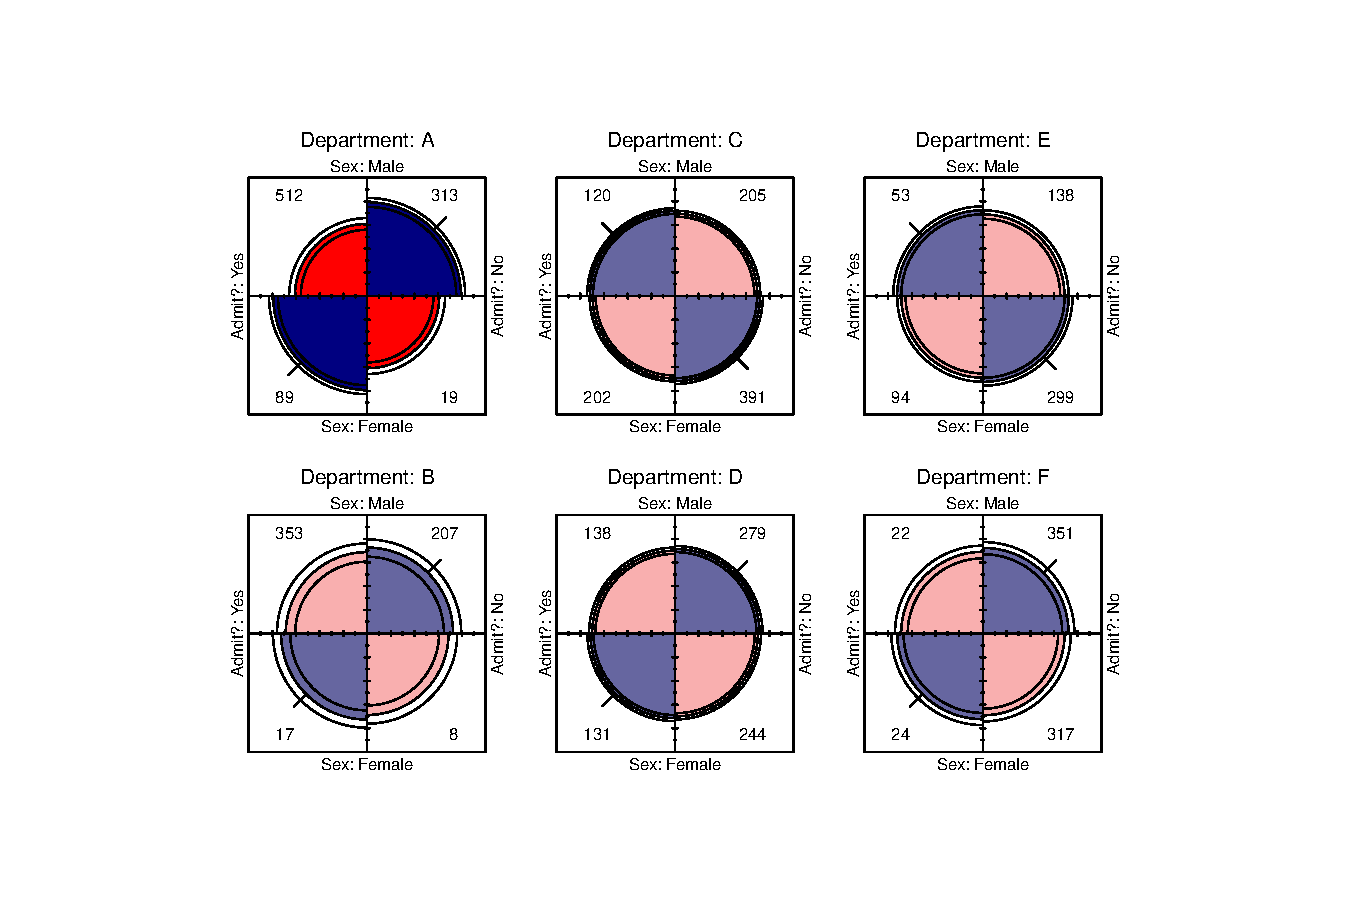
\includegraphics[width=0.8\textwidth,trim=80 50 80 50]{fig/vcd-tut-fourfold1}
\caption{Fourfold display for the \data{UCBAdmissions} data. Where the odds ratio differs
	significantly from 1.0, the confidence bands do not overlap, and the circle quadrants are
	shaded more intensely.}
\label{fig:fourfold1}
\end{center}
\end{figure}

Another \pkg{vcd} function, \codefun{cotabplot}, provides a more general approach
to visualizing conditional associations in contingency tables,
similar to trellis-like plots produced by \codefun{coplot} and lattice graphics.
The \code{panel} argument supplies a function used to render each conditional 
subtable. The following gives a display (not shown) similar to \figref{fig:fourfold1}.
\begin{knitrout}
\definecolor{shadecolor}{rgb}{0.969, 0.969, 0.969}\color{fgcolor}\begin{kframe}
\begin{alltt}
\hlkwd{cotabplot}\hlstd{(UCB,} \hlkwc{panel} \hlstd{= cotab_fourfold)}
\end{alltt}
\end{kframe}
\end{knitrout}


When we want to view the conditional
probabilities of a response variable (e.g., \code{Admit})
in relation to several factors,
an alternative visualization is a \codefun{doubledecker} plot.
This plot is a specialized version of a mosaic plot, which
highlights the levels of a response variable (plotted vertically)
in relation to the factors (shown horizontally). The following
call produces \figref{fig:doubledecker}, where we use indexing
on the first factor (\code{Admit}) to make \code{Admitted}
the highlighted level.

In this plot, the
association between \code{Admit} and \code{Gender} is shown
where the heights of the highlighted conditional probabilities
do not align. The excess of females admitted in Dept A stands out here.

\begin{knitrout}
\definecolor{shadecolor}{rgb}{0.969, 0.969, 0.969}\color{fgcolor}\begin{kframe}
\begin{alltt}
\hlkwd{doubledecker}\hlstd{(Admit} \hlopt{~} \hlstd{Dept} \hlopt{+} \hlstd{Gender,} \hlkwc{data}\hlstd{=UCBAdmissions[}\hlnum{2}\hlopt{:}\hlnum{1}\hlstd{,,])}
\end{alltt}
\end{kframe}
\end{knitrout}


\begin{figure}[htb]
\begin{center}
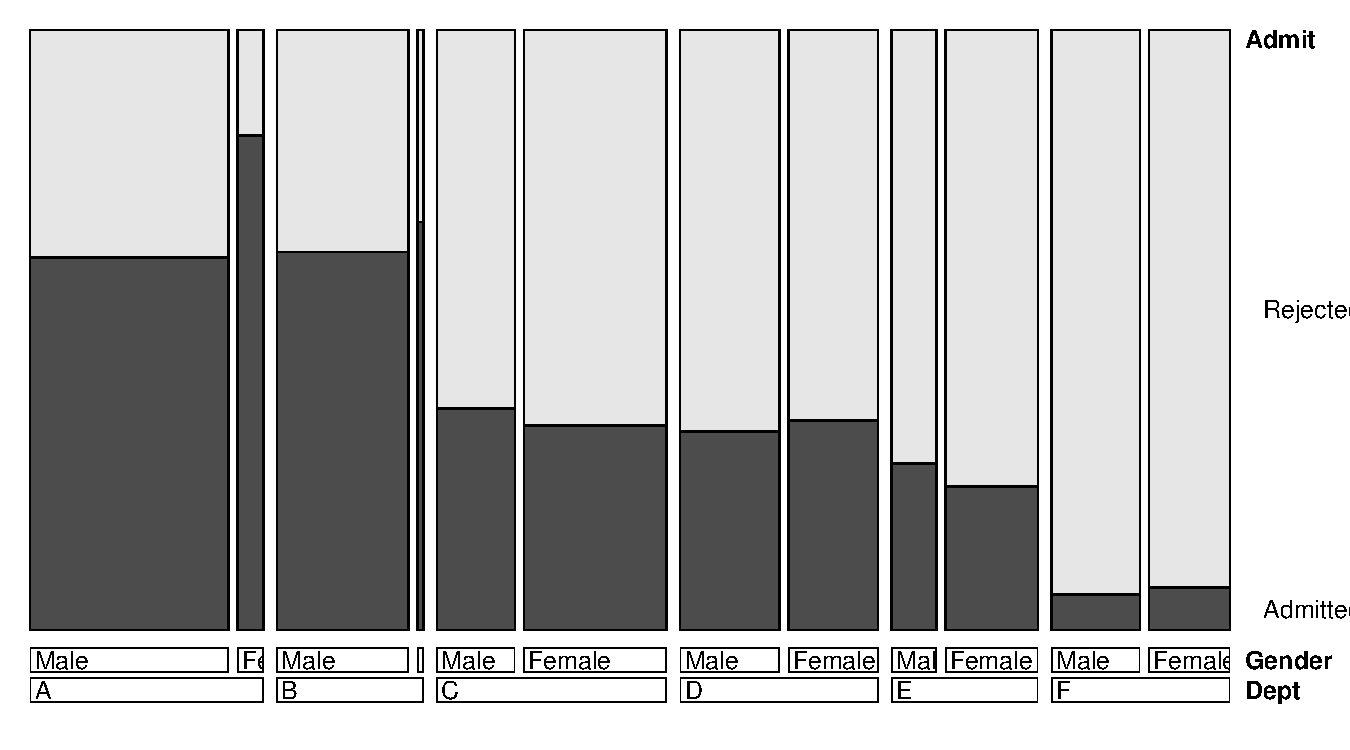
\includegraphics[width=0.9\textwidth]{fig/vcd-tut-doubledecker}
\caption{Doubledecker display for the \data{UCBAdmissions} data. The heights
of the highlighted bars show the conditional probabilities of \texttt{Admit},
given \texttt{Dept} and \texttt{Gender}.}
\label{fig:doubledecker}
\end{center}
\end{figure}

Finally, the there is a \codefun{plot} method for \code{oddsratio} objects.
By default, it shows the 95\% confidence interval for the log odds ratio.
\figref{fig:oddsratio} is produced by \code{plot(lor)}: 
\begin{knitrout}
\definecolor{shadecolor}{rgb}{0.969, 0.969, 0.969}\color{fgcolor}\begin{kframe}
\begin{alltt}
\hlkwd{plot}\hlstd{(lor,} \hlkwc{xlab}\hlstd{=}\hlstr{"Department"}\hlstd{,} \hlkwc{ylab}\hlstd{=}\hlstr{"Log Odds Ratio (Admit | Gender)"}\hlstd{)}
\end{alltt}
\end{kframe}
\end{knitrout}


\begin{figure}[htb]
\begin{center}
%<<oddsratio,fig.height=6,fig.width=6,echo=FALSE>>=
%plot(lor, xlab="Department", ylab="Log Odds Ratio (Admit | Gender)")
%@
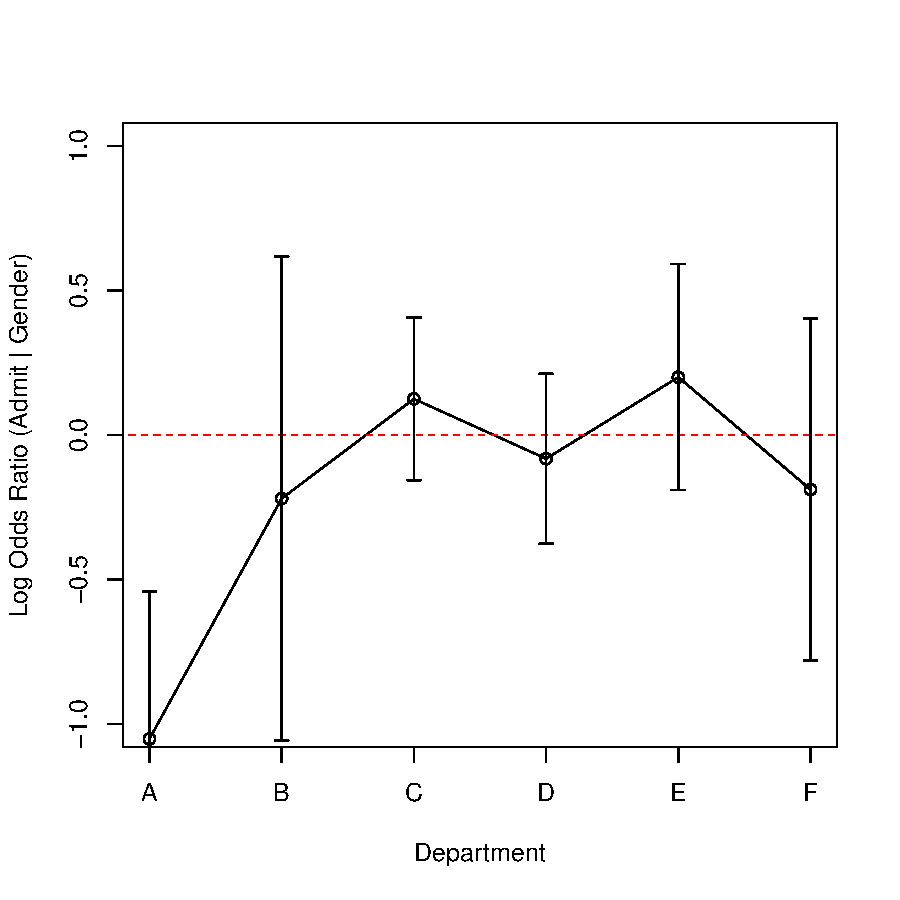
\includegraphics[width=0.5\textwidth]{fig/vcd-tut-oddsratio}
\caption{Log odds ratio plot for the \data{UCBAdmissions} data with 95\% confidence intervals.}
\label{fig:oddsratio}
\end{center}
\end{figure}

\subsection[CMH tests: ordinal factors]{Cochran-Mantel-Haenszel tests for ordinal factors}\label{sec:CMH}
The standard $\chi^2$ tests for association in a two-way table
treat both table factors as nominal (unordered) categories.
When one or both factors of a two-way table are
quantitative or ordinal, more powerful tests of association
may be obtaianed by taking ordinality into account, using
row and or column scores to test for linear trends or differences
in row or column means.

More general versions of the CMH tests (Landis etal., 1978) are provided by assigning
numeric scores to the row and/or column variables. 
For example, with two ordinal factors (assumed to be equally spaced), assigning
integer scores, \code{1:R} and \code{1:C} tests the linear $\times$ linear component
of association. This is statistically equivalent to the Pearson correlation between the
integer-scored table variables, with $\chi^2 = (n-1) r^2$, with only 1 $df$
rather than $(R-1)\times(C-1)$ for the test of general association.

When only one table
variable is ordinal, these general CMH tests are analogous to an ANOVA, testing
whether the row mean scores or column mean scores are equal, again consuming
fewer $df$ than the test of general association.

The \codefun{CMHtest} function in \pkg{vcdExtra} now calculates these various
CMH tests for two possibly ordered factors, optionally stratified other factor(s).

\Example
Recall the $4 \times 4$ table, \code{JobSat} introduced in \secref{sec:creating},
\begin{knitrout}
\definecolor{shadecolor}{rgb}{0.969, 0.969, 0.969}\color{fgcolor}\begin{kframe}
\begin{alltt}
\hlstd{JobSat}
\end{alltt}
\begin{verbatim}
##         satisfaction
## income   VeryD LittleD ModerateS VeryS
##   < 15k      1       3        10     6
##   15-25k     2       3        10     7
##   25-40k     1       6        14    12
##   > 40k      0       1         9    11
\end{verbatim}
\end{kframe}
\end{knitrout}


Treating the \code{satisfaction} levels as equally spaced, but using
midpoints of the \code{income} categories as row scores gives the following results:
\begin{knitrout}
\definecolor{shadecolor}{rgb}{0.969, 0.969, 0.969}\color{fgcolor}\begin{kframe}
\begin{alltt}
\hlkwd{CMHtest}\hlstd{(JobSat,} \hlkwc{rscores}\hlstd{=}\hlkwd{c}\hlstd{(}\hlnum{7.5}\hlstd{,}\hlnum{20}\hlstd{,}\hlnum{32.5}\hlstd{,}\hlnum{60}\hlstd{))}
\end{alltt}
\begin{verbatim}
## Cochran-Mantel-Haenszel Statistics for income by satisfaction 
## 
##                  AltHypothesis Chisq Df  Prob
## cor        Nonzero correlation  3.81  1 0.051
## cmeans  Col mean scores differ  4.48  3 0.214
## rmeans  Row mean scores differ  3.84  3 0.279
## general    General association  5.90  9 0.750
\end{verbatim}
\end{kframe}
\end{knitrout}


Note that with the relatively small cell frequencies, the test for general 
give no evidence for association. However, the the \code{cor} test for linear x linear
association on 1 df is nearly significant. The \pkg{coin} contains the
functions \verb|cmh_test()| and \verb|lbl_test()|
for CMH tests of general association and linear x linear association respectively.

\subsection{Measures of Association}

There are a variety of statistical measures of \emph{strength} of association for
contingency tables--- similar in spirit to $r$ or $r^2$ for continuous variables.
With a large sample size, even a small degree of association can show a 
significant $\chi^2$, as in the example below for the \data{GSS} data.

The  \codefun{assocstats}  function in \pkg{vcd}  calculates  the   $\phi$
contingency coefficient,  and Cramer's  V for  an $r \times c$  table. 
The input must be in table form, a two-way $r \times c$ table.  
It won't work with \data{GSS} in frequency form, but by now you should know how
to convert.
\begin{knitrout}
\definecolor{shadecolor}{rgb}{0.969, 0.969, 0.969}\color{fgcolor}\begin{kframe}
\begin{alltt}
\hlkwd{assocstats}\hlstd{(GSStab)}
\end{alltt}
\begin{verbatim}
##                     X^2 df P(> X^2)
## Likelihood Ratio 7.0026  2 0.030158
## Pearson          7.0095  2 0.030054
## 
## Phi-Coefficient   : 0.085 
## Contingency Coeff.: 0.084 
## Cramer's V        : 0.085
\end{verbatim}
\end{kframe}
\end{knitrout}


For tables with ordinal variables, like \data{JobSat}, some people prefer the
Goodman-Kruskal $\gamma$ statistic (\citet[\S 2.4.3]{vcd:Agresti:2002})
based on a comparison of concordant
and discordant pairs of observations in the case-form equivalent of a two-way table.
\begin{knitrout}
\definecolor{shadecolor}{rgb}{0.969, 0.969, 0.969}\color{fgcolor}\begin{kframe}
\begin{alltt}
\hlkwd{GKgamma}\hlstd{(JobSat)}
\end{alltt}
\begin{verbatim}
## gamma        : 0.221 
## std. error   : 0.117 
## CI           : -0.009 0.451
\end{verbatim}
\end{kframe}
\end{knitrout}


A web article by Richard Darlington,
\url{http://www.psych.cornell.edu/Darlington/crosstab/TABLE0.HTM}
gives further description of these and other measures of association.

\subsection{Measures of Agreement}
The
\codefun{Kappa} function in the \pkg{vcd} package calculates Cohen's $\kappa$ and weighted
$\kappa$ for a square two-way table with the same row and column categories \citep{Cohen:60}.%
\footnote{ 
Don't confuse this with \codefun{kappa} in base \proglang{R} that computes something
entirely different (the condition number of a matrix).
}
Normal-theory $z$-tests are obtained by dividing $\kappa$ by its asymptotic standard
error (ASE).  A \codefun{confint} method for \code{Kappa} objects provides confidence intervals.
\begin{knitrout}
\definecolor{shadecolor}{rgb}{0.969, 0.969, 0.969}\color{fgcolor}\begin{kframe}
\begin{alltt}
\hlstd{(K} \hlkwb{<-} \hlkwd{Kappa}\hlstd{(SexualFun))}
\end{alltt}
\begin{verbatim}
##            value    ASE    z
## Unweighted 0.129 0.0688 1.88
## Weighted   0.237 0.1265 1.88
\end{verbatim}
\begin{alltt}
\hlkwd{confint}\hlstd{(K)}
\end{alltt}
\begin{verbatim}
##             
## Kappa              lwr    upr
##   Unweighted -0.005605 0.2643
##   Weighted   -0.010487 0.4852
\end{verbatim}
\end{kframe}
\end{knitrout}


A visualization of agreement, both unweighted and weighted for degree of departure
from exact agreement is provided by the \codefun{agreementplot} function.
\figref{fig:agreesex} shows the agreementplot for the \data{SexualFun} data,
produced as shown below. The Bangdiwala measures represent the proportion of the
shaded areas of the diagonal rectangles, using weights $w_1$ for exact agreement,
and $w_2$ for partial agreement one step from the main diagonal.
\begin{knitrout}
\definecolor{shadecolor}{rgb}{0.969, 0.969, 0.969}\color{fgcolor}\begin{kframe}
\begin{alltt}
\hlstd{agree} \hlkwb{<-} \hlkwd{agreementplot}\hlstd{(SexualFun,} \hlkwc{main}\hlstd{=}\hlstr{"Is sex fun?"}\hlstd{)}
\hlkwd{unlist}\hlstd{(agree)}
\end{alltt}
\begin{verbatim}
##          Bangdiwala Bangdiwala_Weighted            weights1 
##              0.1465              0.4982              1.0000 
##            weights2 
##              0.8889
\end{verbatim}
\end{kframe}
\end{knitrout}


\begin{figure}[htb]
\begin{center}
%<<agreesex,fig=TRUE,height=6,width=7,results='markup'>>=
%agree <- agreementplot(SexualFun, main="Is sex fun?")
%agree
%@
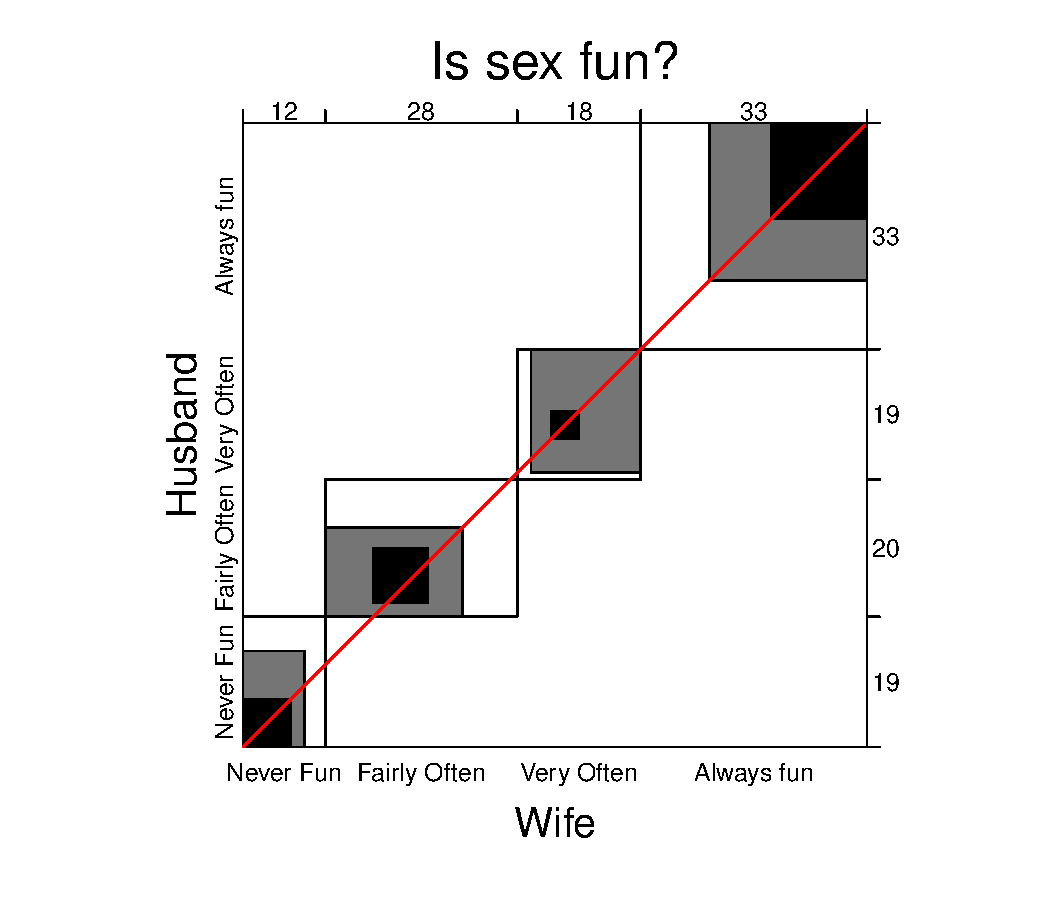
\includegraphics[width=0.4\textwidth,trim=50 25 50 25]{fig/vcd-tut-agreesex}
\caption{Agreement plot for the \data{SexualFun} data.}
\label{fig:agreesex}
\end{center}
\end{figure}
In other examples, the agreement plot can help to show \emph{sources}
of disagreement.  For example, when the shaded boxes are above or below the diagonal
(red) line, a lack of exact agreement can be attributed in part to
different frequency of use of categories by the two raters-- lack of
\emph{marginal homogeneity}.
	
\subsection{Correspondence analysis}
Use the \pkg{ca} package for correspondence analysis for visually exploring relationships
between rows and columns in contingency tables.  For an $r \times c$ table,
the method provides a breakdown of the Pearson $\chi^2$ for association in up to $M = \min(r-1, c-1)$
dimensions, and finds scores for the row ($x_{im}$) and column ($y_{jm}$) categories
such that the observations have the maximum possible correlations.%
\footnote{
	Related methods are the non-parametric
	CMH tests using assumed row/column scores (\secref{sec:CMH}),
	the analogous \codefun{glm} model-based methods (\secref{sec:CMH}),
	and the more general RC models which can be fit using \codefun{gnm}.
	Correspondence analysis differs in that it is a primarily
	descriptive/exploratory method (no significance tests), but is
	directly tied to informative graphic displays of the row/column categories.
}	
	


Here, we carry out a simple correspondence analysis of the \data{HairEye} data.
The printed results show that nearly 99\% of the association between hair color and eye color
can be accounted for in 2 dimensions, of which the first dimension accounts for 90\%.
\begin{knitrout}
\definecolor{shadecolor}{rgb}{0.969, 0.969, 0.969}\color{fgcolor}\begin{kframe}
\begin{alltt}
\hlkwd{library}\hlstd{(ca)}
\hlkwd{ca}\hlstd{(HairEye)}
\end{alltt}
\begin{verbatim}
## 
##  Principal inertias (eigenvalues):
##            1        2        3       
## Value      0.208773 0.022227 0.002598
## Percentage 89.37%   9.52%    1.11%   
## 
## 
##  Rows:
##            Black    Brown     Red  Blond
## Mass     0.18243  0.48311  0.1199 0.2145
## ChiDist  0.55119  0.15946  0.3548 0.8384
## Inertia  0.05543  0.01228  0.0151 0.1508
## Dim. 1  -1.10428 -0.32446 -0.2835 1.8282
## Dim. 2   1.44092 -0.21911 -2.1440 0.4667
## 
## 
##  Columns:
##            Brown    Hazel    Green   Blue
## Mass     0.37162  0.15710  0.10811 0.3632
## ChiDist  0.50049  0.28865  0.38573 0.5537
## Inertia  0.09309  0.01309  0.01608 0.1113
## Dim. 1  -1.07713 -0.46529  0.35401 1.1981
## Dim. 2   0.59242 -1.12278 -2.27412 0.5564
\end{verbatim}
\end{kframe}
\end{knitrout}


The resulting \code{ca} object can be plotted just by running the \codefun{plot}
method on the \code{ca} object, giving the result in
\figref{fig:ca-haireye}.  \codefun{plot.ca} does not allow labels for dimensions;
these can be added with \codefun{title}.
It can be seen that most of the association is accounted for by the ordering
of both hair color and eye color along Dimension 1, a dark to light dimension.
\begin{knitrout}
\definecolor{shadecolor}{rgb}{0.969, 0.969, 0.969}\color{fgcolor}\begin{kframe}
\begin{alltt}
\hlkwd{plot}\hlstd{(}\hlkwd{ca}\hlstd{(HairEye),} \hlkwc{main}\hlstd{=}\hlstr{"Hair Color and Eye Color"}\hlstd{)}
\hlkwd{title}\hlstd{(}\hlkwc{xlab}\hlstd{=}\hlstr{"Dim 1 (89.4%)"}\hlstd{,} \hlkwc{ylab}\hlstd{=}\hlstr{"Dim 2 (9.5%)"}\hlstd{)}
\end{alltt}
\end{kframe}
\end{knitrout}


\begin{figure}[htb]
\begin{center}
%<<ca-haireye,results='hide',echo=FALSE>>=
%plot(ca(HairEye), main="Hair Color and Eye Color")
%title(xlab="Dim 1 (89.4%)", ylab="Dim 2 (9.5%)")
%@
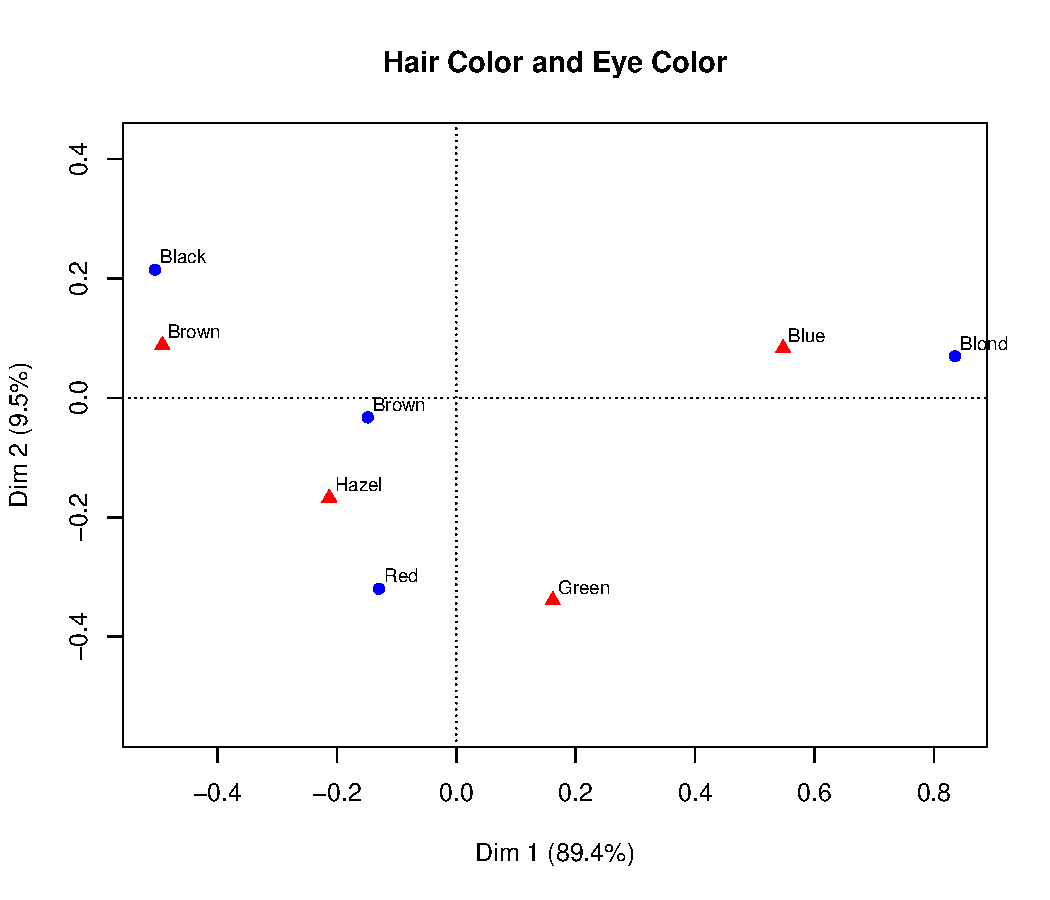
\includegraphics[width=0.7\textwidth]{fig/vcd-tut-ca-haireye}
\caption{Correspondence analysis plot for the \data{HairEye} data.}
\label{fig:ca-haireye}
\end{center}
\end{figure}

\section{Loglinear Models}\label{sec:loglin}

You can  use the  \codefun{loglm}  function in  the \pkg{MASS}  package to fit log-linear
models.  Equivalent models can also be fit (from a different perspective) as generalized
linear models with the \codefun{glm}  function using the \code{family='poisson'} argument,
and the \pkg{gnm} package provides a wider range of generalized \emph{nonlinear} models,
particularly for testing structured associations.
The visualization methods for these models were originally developed for models fit using \codefun{loglm},
so this approach is emphasized here.  Some extensions of these methods for models
fit using \codefun{glm} and \codefun{gnm} are contained in the \pkg{vcdExtra} package
and illustrated in \secref{sec:glm}.

Assume we  have a 3-way  contingency table based  on
variables A, B, and C.  
The possible different forms of \loglin\ models for a 3-way table are shown in \tabref{tab:loglin-3way}.
The \textbf{Model formula} column shows how to express each model for \codefun{loglm} in \proglang{R}.%
\footnote{
For \codefun{glm}, or \codefun{gnm}, with the data in the form of a frequency data.frame, the same model is specified
in the form \code{glm(Freq} $\sim$ \code{..., family="poisson")}, where \texttt{Freq} is  the name
of the cell frequency variable and \texttt{...} specifies the \textbf{Model formula}.
}
In the \textbf{Interpretation} column, the symbol ``$\perp$'' is to be read as ``is independent of,''
and ``$\given$'' means ``conditional on,'' or ``adjusting for,'' or just ``given''.

\begin{table}[htb]
 \caption{Log-linear Models for Three-Way Tables}\label{tab:loglin-3way}
 \begin{center}
 \begin{tabular}{llll}
  \hline
  \textbf{Model}           & \textbf{Model formula}  & \textbf{Symbol}& \textbf{Interpretation} \\
  \hline\hline 
  Mutual independence      & \verb|~A + B + C|       & $[A][B][C]$    & $A \perp B \perp C$ \\ 
  Joint independence       & \verb|~A*B + C|         & $[AB][C]$      & $(A \: B) \perp C$ \\ 
  Conditional independence & \verb|~(A+B)*C|         & $[AC][BC]$     & $(A \perp B) \given C$ \\ 
  All two-way associations & \verb|~A*B + A*C + B*C| & $[AB][AC][BC]$ & homogeneous association  \\ 
  Saturated model          & \verb|~A*B*C|           & $[ABC]$        & 3-way association \\ 
  \hline
 \end{tabular}
 \end{center}
\end{table}



For example, the formula \verb|~A + B + C| specifies the model of \emph{mutual independence} with
no associations among the three factors.  In standard notation for the expected frequencies
$m_{ijk}$, this corresponds to
\begin{equation*}
	\log ( m_{ijk} ) = \mu + \lambda_i^A + \lambda_j^B + \lambda_k^C \equiv \texttt{A + B + C}
\end{equation*}
The parameters $\lambda_i^A , \lambda_j^B$ and  $\lambda_k^C$ pertain to the differences among the
one-way marginal frequencies for the factors A, B and C. 

Similarly, the model of \emph{joint independence},  $(A \: B) \perp C$,
allows an association between A and B, but specifies that
C is independent of both of these and their combinations,
\begin{equation*}
	\log ( m_{ijk} ) = \mu + \lambda_i^A + \lambda_j^B + \lambda_k^C + \lambda_{ij}^{AB} \equiv \texttt{A * B + C}
\end{equation*}
where the parameters $\lambda_{ij}^{AB}$ pertain to the overall association between A and B (collapsing over C).

In the literature or text books, you will often find these models expressed in shorthand symbolic notation,
using brackets, \texttt{[ ]} to enclose the \emph{high-order terms} in the model.
Thus, the joint independence model can be denoted \texttt{[AB][C]}, as shown in the \textbf{Symbol} column in 
\tabref{tab:loglin-3way}.

Models of \emph{conditional independence} allow (and fit)  two of the three possible
two-way associations.  There are three such models, depending on which variable is conditioned upon.
For a given conditional independence model, e.g., \texttt{[AB][AC]}, the given variable is the one
common to all terms, so this example has the interpretation $(B \perp C) \given A$.


\subsection[Fitting with loglm()]{Fitting with \codefun{loglm}}\label{sec:loglm}
For example, we can fit the model of mutual independence among hair color, eye color and sex 
in \data{HairEyeColor} as

\begin{knitrout}
\definecolor{shadecolor}{rgb}{0.969, 0.969, 0.969}\color{fgcolor}\begin{kframe}
\begin{alltt}
\hlkwd{library}\hlstd{(MASS)}
\hlcom{## Independence model of hair and eye color and sex.  }
\hlstd{hec.1} \hlkwb{<-} \hlkwd{loglm}\hlstd{(}\hlopt{~}\hlstd{Hair}\hlopt{+}\hlstd{Eye}\hlopt{+}\hlstd{Sex,} \hlkwc{data}\hlstd{=HairEyeColor)}
\hlstd{hec.1}
\end{alltt}
\begin{verbatim}
## Call:
## loglm(formula = ~Hair + Eye + Sex, data = HairEyeColor)
## 
## Statistics:
##                    X^2 df P(> X^2)
## Likelihood Ratio 166.3 24        0
## Pearson          164.9 24        0
\end{verbatim}
\end{kframe}
\end{knitrout}


Similarly, the models of conditional independence (\code{hec.2}) 
and joint independence (\code{hec.3}) are specified as
\begin{knitrout}
\definecolor{shadecolor}{rgb}{0.969, 0.969, 0.969}\color{fgcolor}\begin{kframe}
\begin{alltt}
\hlcom{## Conditional independence}
\hlstd{hec.2} \hlkwb{<-} \hlkwd{loglm}\hlstd{(}\hlopt{~}\hlstd{(Hair} \hlopt{+} \hlstd{Eye)} \hlopt{*} \hlstd{Sex,} \hlkwc{data}\hlstd{=HairEyeColor)}
\hlstd{hec.2}
\end{alltt}
\begin{verbatim}
## Call:
## loglm(formula = ~(Hair + Eye) * Sex, data = HairEyeColor)
## 
## Statistics:
##                    X^2 df P(> X^2)
## Likelihood Ratio 156.7 18        0
## Pearson          147.9 18        0
\end{verbatim}
\end{kframe}
\end{knitrout}

\begin{knitrout}
\definecolor{shadecolor}{rgb}{0.969, 0.969, 0.969}\color{fgcolor}\begin{kframe}
\begin{alltt}
\hlcom{## Joint independence model.  }
\hlstd{hec.3} \hlkwb{<-} \hlkwd{loglm}\hlstd{(}\hlopt{~}\hlstd{Hair}\hlopt{*}\hlstd{Eye} \hlopt{+} \hlstd{Sex,} \hlkwc{data}\hlstd{=HairEyeColor)}
\hlstd{hec.3}
\end{alltt}
\begin{verbatim}
## Call:
## loglm(formula = ~Hair * Eye + Sex, data = HairEyeColor)
## 
## Statistics:
##                    X^2 df P(> X^2)
## Likelihood Ratio 19.86 15   0.1775
## Pearson          19.57 15   0.1892
\end{verbatim}
\end{kframe}
\end{knitrout}

Note that printing the model gives a brief summary of the goodness of fit.
A set of models can be compared using the \codefun{anova} function.

\begin{knitrout}
\definecolor{shadecolor}{rgb}{0.969, 0.969, 0.969}\color{fgcolor}\begin{kframe}
\begin{alltt}
\hlkwd{anova}\hlstd{(hec.1, hec.2, hec.3)}
\end{alltt}
\begin{verbatim}
## LR tests for hierarchical log-linear models
## 
## Model 1:
##  ~Hair + Eye + Sex 
## Model 2:
##  ~(Hair + Eye) * Sex 
## Model 3:
##  ~Hair * Eye + Sex 
## 
##           Deviance df Delta(Dev) Delta(df) P(> Delta(Dev)
## Model 1     166.30 24                                    
## Model 2     156.68 18      9.622         6         0.1415
## Model 3      19.86 15    136.821         3         0.0000
## Saturated     0.00  0     19.857        15         0.1775
\end{verbatim}
\end{kframe}
\end{knitrout}


\pkg{vcdExtra} now provides a convenience function \codefun{loglmlist}
for collecting a set of related log-linear models into a list, of class
\class{loglmlist}, with \code{summarise} and \code{mosaic} methods.  For 
example, an abbreviated ANOVA table for these models is produced by
\begin{knitrout}
\definecolor{shadecolor}{rgb}{0.969, 0.969, 0.969}\color{fgcolor}\begin{kframe}
\begin{alltt}
\hlstd{vcdExtra::}\hlkwd{summarise}\hlstd{(}\hlkwd{loglmlist}\hlstd{(hec.1, hec.2, hec.3))}
\end{alltt}
\begin{verbatim}
## Re-fitting to get fitted values
## Re-fitting to get fitted values
## Re-fitting to get fitted values
## Model Summary:
##       LR Chisq Df Pr(>Chisq)   AIC   BIC
## hec.1    166.3 24      0.000 118.3  13.1
## hec.2    156.7 18      0.000 120.7  41.8
## hec.3     19.9 15      0.177 -10.1 -75.9
\end{verbatim}
\end{kframe}
\end{knitrout}


%Martin Theus and Stephan Lauer have written an excellent article on  Visualizing
%Loglinear Models, using  mosaic plots. There  is also great  tutorial example by
%Kevin Quinn on analyzing loglinear models via glm.

\subsection[Fitting with glm() and gnm()]{Fitting with \codefun{glm} and \codefun{gnm}}\label{sec:glm}
The \codefun{glm} approach, and extensions of this in the \pkg{gnm} package allows a
much wider class of models for frequency data to be fit than can be handled by
\codefun{loglm}.  Of particular importance are models for ordinal factors and for
square tables, where we can test more structured hypotheses about the patterns
of association than are provided in the tests of general assosiation under
\codefun{loglm}. These are similar in spirit to the 
non-parametric CMH tests described in \secref{sec:CMH}.

\Example
The data \code{Mental} in the \pkg{vcdExtra} package gives a two-way table in frequency form
classifying young people by
their mental health status and parents' socioeconomic status (SES), where
both of these variables are ordered factors.
\begin{knitrout}
\definecolor{shadecolor}{rgb}{0.969, 0.969, 0.969}\color{fgcolor}\begin{kframe}
\begin{alltt}
\hlkwd{str}\hlstd{(Mental)}
\end{alltt}
\begin{verbatim}
## 'data.frame':	24 obs. of  3 variables:
##  $ ses   : Ord.factor w/ 6 levels "1"<"2"<"3"<"4"<..: 1 1 1 1 2 2 2 2 3 3 ...
##  $ mental: Ord.factor w/ 4 levels "Well"<"Mild"<..: 1 2 3 4 1 2 3 4 1 2 ...
##  $ Freq  : int  64 94 58 46 57 94 54 40 57 105 ...
\end{verbatim}
\begin{alltt}
\hlkwd{xtabs}\hlstd{(Freq} \hlopt{~} \hlstd{mental}\hlopt{+}\hlstd{ses,} \hlkwc{data}\hlstd{=Mental)}   \hlcom{# display the frequency table}
\end{alltt}
\begin{verbatim}
##           ses
## mental       1   2   3   4   5   6
##   Well      64  57  57  72  36  21
##   Mild      94  94 105 141  97  71
##   Moderate  58  54  65  77  54  54
##   Impaired  46  40  60  94  78  71
\end{verbatim}
\end{kframe}
\end{knitrout}

Simple ways of handling ordinal variables involve assigning scores to the table
categories, and the simplest cases are to use integer scores, either for the row variable (``column
effects'' model), the column variable (``row effects'' model), or both (``uniform association''
model).

\begin{knitrout}
\definecolor{shadecolor}{rgb}{0.969, 0.969, 0.969}\color{fgcolor}\begin{kframe}
\begin{alltt}
\hlstd{indep} \hlkwb{<-} \hlkwd{glm}\hlstd{(Freq} \hlopt{~} \hlstd{mental} \hlopt{+} \hlstd{ses,} \hlkwc{family} \hlstd{= poisson,} \hlkwc{data} \hlstd{= Mental)}  \hlcom{# independence model}
\end{alltt}
\end{kframe}
\end{knitrout}

To fit more parsimonious models than general association, we can define
numeric scores for the row and column categories
\begin{knitrout}
\definecolor{shadecolor}{rgb}{0.969, 0.969, 0.969}\color{fgcolor}\begin{kframe}
\begin{alltt}
\hlcom{# Use integer scores for rows/cols }
\hlstd{Cscore} \hlkwb{<-} \hlkwd{as.numeric}\hlstd{(Mental}\hlopt{$}\hlstd{ses)}
\hlstd{Rscore} \hlkwb{<-} \hlkwd{as.numeric}\hlstd{(Mental}\hlopt{$}\hlstd{mental)}
\end{alltt}
\end{kframe}
\end{knitrout}

Then, the row effects model, the column effects model, and the uniform association
model can be fit as follows:
\begin{knitrout}
\definecolor{shadecolor}{rgb}{0.969, 0.969, 0.969}\color{fgcolor}\begin{kframe}
\begin{alltt}
\hlcom{# column effects model (ses)}
\hlstd{coleff} \hlkwb{<-} \hlkwd{glm}\hlstd{(Freq} \hlopt{~} \hlstd{mental} \hlopt{+} \hlstd{ses} \hlopt{+} \hlstd{Rscore}\hlopt{:}\hlstd{ses,} \hlkwc{family} \hlstd{= poisson,} \hlkwc{data} \hlstd{= Mental)}
\hlcom{# row effects model (mental)}
\hlstd{roweff} \hlkwb{<-} \hlkwd{glm}\hlstd{(Freq} \hlopt{~} \hlstd{mental} \hlopt{+} \hlstd{ses} \hlopt{+} \hlstd{mental}\hlopt{:}\hlstd{Cscore,} \hlkwc{family} \hlstd{= poisson,} \hlkwc{data} \hlstd{= Mental)}
\hlcom{# linear x linear association}
\hlstd{linlin} \hlkwb{<-} \hlkwd{glm}\hlstd{(Freq} \hlopt{~} \hlstd{mental} \hlopt{+} \hlstd{ses} \hlopt{+} \hlstd{Rscore}\hlopt{:}\hlstd{Cscore,} \hlkwc{family} \hlstd{= poisson,} \hlkwc{data} \hlstd{= Mental)}
\end{alltt}
\end{kframe}
\end{knitrout}

The \codefun{summarize} function in \pkg{vcdExtra} provides a nice, compact summary of the
fit statistics for a set of models, collected into a \class{glmlist} object.
Smaller is better for AIC and BIC.
\begin{knitrout}
\definecolor{shadecolor}{rgb}{0.969, 0.969, 0.969}\color{fgcolor}\begin{kframe}
\begin{alltt}
\hlcom{# compare models using AIC, BIC, etc}
\hlstd{vcdExtra::}\hlkwd{summarise}\hlstd{(}\hlkwd{glmlist}\hlstd{(indep, roweff, coleff, linlin))}
\end{alltt}
\begin{verbatim}
## Model Summary:
##        LR Chisq Df Pr(>Chisq)   AIC   BIC
## indep      47.4 15      0.000  17.4 -63.8
## roweff      6.3 12      0.901 -17.7 -82.7
## coleff      6.8 10      0.741 -13.2 -67.3
## linlin      9.9 14      0.770 -18.1 -93.9
\end{verbatim}
\end{kframe}
\end{knitrout}

For specific model comparisons, we can also carry out tests of \emph{nested} models with
\codefun{anova} when those models are listed from smallest to largest.
Here, there are two separate paths from the most restrictive (independence) model
through the model of uniform association, to those that allow only one of
row effects or column effects.
\begin{knitrout}
\definecolor{shadecolor}{rgb}{0.969, 0.969, 0.969}\color{fgcolor}\begin{kframe}
\begin{alltt}
\hlkwd{anova}\hlstd{(indep, linlin, coleff,} \hlkwc{test}\hlstd{=}\hlstr{"Chisq"}\hlstd{)}
\end{alltt}
\begin{verbatim}
## Analysis of Deviance Table
## 
## Model 1: Freq ~ mental + ses
## Model 2: Freq ~ mental + ses + Rscore:Cscore
## Model 3: Freq ~ mental + ses + Rscore:ses
##   Resid. Df Resid. Dev Df Deviance Pr(>Chi)    
## 1        15       47.4                         
## 2        14        9.9  1     37.5    9e-10 ***
## 3        10        6.8  4      3.1     0.55    
## ---
## Signif. codes:  0 '***' 0.001 '**' 0.01 '*' 0.05 '.' 0.1 ' ' 1
\end{verbatim}
\begin{alltt}
\hlkwd{anova}\hlstd{(indep, linlin, roweff,} \hlkwc{test}\hlstd{=}\hlstr{"Chisq"}\hlstd{)}
\end{alltt}
\begin{verbatim}
## Analysis of Deviance Table
## 
## Model 1: Freq ~ mental + ses
## Model 2: Freq ~ mental + ses + Rscore:Cscore
## Model 3: Freq ~ mental + ses + mental:Cscore
##   Resid. Df Resid. Dev Df Deviance Pr(>Chi)    
## 1        15       47.4                         
## 2        14        9.9  1     37.5    9e-10 ***
## 3        12        6.3  2      3.6     0.16    
## ---
## Signif. codes:  0 '***' 0.001 '**' 0.01 '*' 0.05 '.' 0.1 ' ' 1
\end{verbatim}
\end{kframe}
\end{knitrout}

The model of linear by linear association seems best on all accounts.
For comparison, one might try the CMH tests on these data:

\begin{knitrout}
\definecolor{shadecolor}{rgb}{0.969, 0.969, 0.969}\color{fgcolor}\begin{kframe}
\begin{alltt}
\hlkwd{CMHtest}\hlstd{(}\hlkwd{xtabs}\hlstd{(Freq}\hlopt{~}\hlstd{ses}\hlopt{+}\hlstd{mental,} \hlkwc{data}\hlstd{=Mental))}
\end{alltt}
\begin{verbatim}
## Cochran-Mantel-Haenszel Statistics for ses by mental 
## 
##                  AltHypothesis Chisq Df     Prob
## cor        Nonzero correlation  37.2  1 1.09e-09
## cmeans  Col mean scores differ  40.3  5 1.30e-07
## rmeans  Row mean scores differ  40.7  3 7.70e-09
## general    General association  46.0 15 5.40e-05
\end{verbatim}
\end{kframe}
\end{knitrout}


\subsection{Non-linear terms}
The strength of the \pkg{gnm} package is that it handles a wide variety of models
that handle non-linear terms, where the parameters enter the model beyond a simple
linear function.
The simplest example is the Goodman RC(1) model, which allows a multiplicative
term to account for the association of the table variables.
In the notation of generalized linear models with a log link, this can be expressed as
\begin{equation*}
\log \mu_{ij} = \alpha_i + \beta_j + \gamma_{i} \delta_{j}	
\end{equation*}
where the row-multiplicative effect parameters $\gamma_i$ and 
corresponding column parameters $\delta_j$ are estimated from the data.%
\footnote{
This is similar in spirit to a correspondence analysis with a single
dimension, but as a statistical model.
}
Similarly, the RC(2) model adds two multiplicative terms to
the independence model,
\begin{equation*}
\log \mu_{ij} = \alpha_i + \beta_j + \gamma_{i1} \delta_{j1} + \gamma_{i2} \delta_{j2}
\end{equation*}

In the \pkg{gnm} package, these models may be fit using the \codefun{Mult}
to specify the multiplicative term, and \codefun{instances} to specify several
such terms.

\Example
For the \code{Mental} data, we fit the RC(1) and RC(2) models, and compare
these with the independence model.

\begin{knitrout}
\definecolor{shadecolor}{rgb}{0.969, 0.969, 0.969}\color{fgcolor}\begin{kframe}
\begin{alltt}
\hlstd{RC1} \hlkwb{<-} \hlkwd{gnm}\hlstd{(Freq} \hlopt{~} \hlstd{mental} \hlopt{+} \hlstd{ses} \hlopt{+} \hlkwd{Mult}\hlstd{(mental,ses),} \hlkwc{data}\hlstd{=Mental,}
             \hlkwc{family}\hlstd{=poisson, ,} \hlkwc{verbose}\hlstd{=}\hlnum{FALSE}\hlstd{)}
\hlstd{RC2} \hlkwb{<-} \hlkwd{gnm}\hlstd{(Freq} \hlopt{~} \hlstd{mental}\hlopt{+}\hlstd{ses} \hlopt{+} \hlkwd{instances}\hlstd{(}\hlkwd{Mult}\hlstd{(mental,ses),}\hlnum{2}\hlstd{),} \hlkwc{data}\hlstd{=Mental,}
             \hlkwc{family}\hlstd{=poisson,} \hlkwc{verbose}\hlstd{=}\hlnum{FALSE}\hlstd{)}
\hlkwd{anova}\hlstd{(indep, RC1, RC2,} \hlkwc{test}\hlstd{=}\hlstr{"Chisq"}\hlstd{)}
\end{alltt}
\begin{verbatim}
## Analysis of Deviance Table
## 
## Model 1: Freq ~ mental + ses
## Model 2: Freq ~ mental + ses + Mult(mental, ses)
## Model 3: Freq ~ mental + ses + Mult(mental, ses, inst = 1) + Mult(mental, 
##     ses, inst = 2)
##   Resid. Df Resid. Dev Df Deviance Pr(>Chi)    
## 1        15       47.4                         
## 2         9       40.2  6      7.2      0.3    
## 3         3        0.5  6     39.7  5.2e-07 ***
## ---
## Signif. codes:  0 '***' 0.001 '**' 0.01 '*' 0.05 '.' 0.1 ' ' 1
\end{verbatim}
\end{kframe}
\end{knitrout}


\section{Mosaic plots}\label{sec:mosaic}

Mosaic plots provide an ideal method both for visualizing contingency tables and for 
visualizing the fit--- or more importantly--- lack of fit of a \loglin\ model.
For a two-way table, \codefun{mosaic} fits a model of independence, $[A][B]$
or \verb|~A+B| as an \proglang{R} formula.
For $n$-way tables, \codefun{mosaic} can fit any \loglin\ model, and can also be
used to plot a model fit with \codefun{loglm}.
See \citet{vcd:Friendly:1994,vcd:Friendly:1999} for the statistical ideas behind these
uses of mosaic displays in connection with \loglin\ models.

The essential idea is to recursively sub-divide a unit square into rectangular ``tiles'' for the
cells of the table, such
that the are area of each tile is proportional to the cell frequency.
For a given \loglin\ model, the tiles can then be shaded in various ways to reflect
the residuals (lack of fit) for a given model.  The pattern of residuals can then
be used to suggest a better model or understand \emph{where} a given model fits or
does not fit.

\codefun{mosaic} provides a wide range of options for the directions of splitting,
the specification of shading, labeling, spacing, legend and many other details.
It is actually implemented as a special case of a more general
class of displays for $n$-way tables called \code{strucplot}, including
sieve diagrams, association plots, double-decker plots as well as mosaic
plots.  For details, see \code{help(strucplot)} and the ``See also'' links,
and also \citet{vcd:Meyer+Zeileis+Hornik:2006b}, which is available as
an \proglang{R} vignette via \code{vignette("strucplot", package="vcd")}.

\figref{fig:arthritis}, showing the association between
\code{Treatment} and \code{Improved} was produced with the following
call to \codefun{mosaic}.
\begin{knitrout}
\definecolor{shadecolor}{rgb}{0.969, 0.969, 0.969}\color{fgcolor}\begin{kframe}
\begin{alltt}
\hlkwd{mosaic}\hlstd{(art,} \hlkwc{gp} \hlstd{= shading_max,} \hlkwc{split_vertical} \hlstd{=} \hlnum{TRUE}\hlstd{,}
       \hlkwc{main}\hlstd{=}\hlstr{"Arthritis: [Treatment] [Improved]"}\hlstd{)}
\end{alltt}
\end{kframe}
\end{knitrout}

Note that the residuals for the independence model were not large
(as shown in the legend),
yet the association between \code{Treatment} and \code{Improved}
is highly significant.
\begin{knitrout}
\definecolor{shadecolor}{rgb}{0.969, 0.969, 0.969}\color{fgcolor}\begin{kframe}
\begin{alltt}
\hlkwd{summary}\hlstd{(art)}
\end{alltt}
\begin{verbatim}
## Call: xtabs(formula = ~Treatment + Improved, data = Arthritis)
## Number of cases in table: 84 
## Number of factors: 2 
## Test for independence of all factors:
## 	Chisq = 13, df = 2, p-value = 0.001
\end{verbatim}
\end{kframe}
\end{knitrout}

In contrast, one of the other shading schemes, from \citet{vcd:Friendly:1994}
(use: \verb|gp = shading_Friendly|), 
uses fixed cutoffs of $\pm 2, \pm 4$,
to shade cells which are \emph{individually} significant
at approximately $\alpha = 0.05$ and $\alpha = 0.001$ levels, respectively.
The right panel below uses \verb|gp = shading_Friendly|.

%\setkeys{Gin}{width=0.5\textwidth}




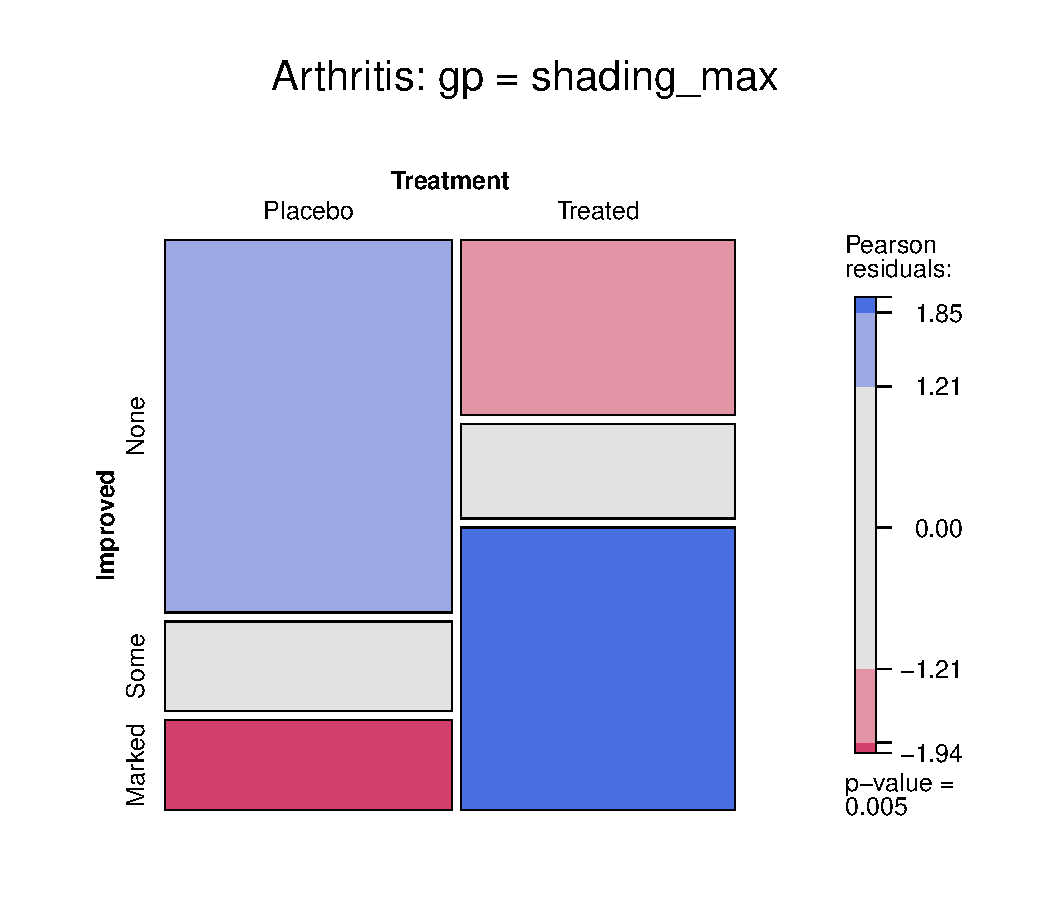
\includegraphics[width=0.49\textwidth]{fig/vcd-tut-art21}
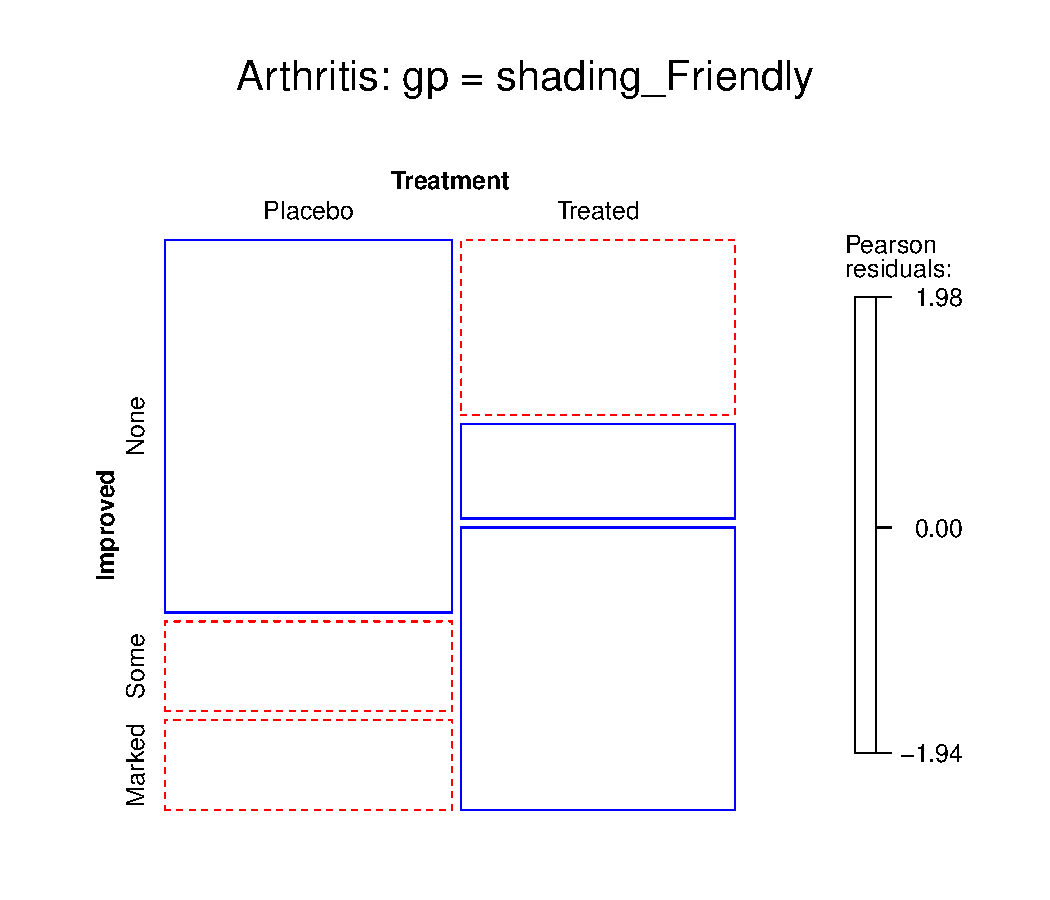
\includegraphics[width=0.49\textwidth]{fig/vcd-tut-art22}


\subsection[Mosaics for loglinear models]{Mosaics for \loglin\ models}\label{sec:mosaic-llm}

When you have fit a \loglin\ model using \codefun{loglm}, 
and saved the result (as a \code{loglm} object) the simplest way to display the
results is to use the \codefun{plot} method for the \code{loglm} object.
Calling \code{mosaic(loglm.object)} has the same result.
In \secref{sec:loglm} above, we fit several different models to the
\data{HairEyeColor} data.  We can produce mosaic displays of each just
by plotting them:

\begin{knitrout}
\definecolor{shadecolor}{rgb}{0.969, 0.969, 0.969}\color{fgcolor}\begin{kframe}
\begin{alltt}
\hlcom{# mosaic plots, using plot.loglm() method}
\hlkwd{plot}\hlstd{(hec.1,} \hlkwc{main}\hlstd{=}\hlstr{"model: [Hair][Eye][Sex]"}\hlstd{)}
\hlkwd{plot}\hlstd{(hec.2,} \hlkwc{main}\hlstd{=}\hlstr{"model: [HairSex][EyeSex]"}\hlstd{)}
\hlkwd{plot}\hlstd{(hec.3,} \hlkwc{main}\hlstd{=}\hlstr{"model: [HairEye][Sex]"}\hlstd{)}
\end{alltt}
\end{kframe}
\end{knitrout}


%\setkeys{Gin}{width=0.32\textwidth}






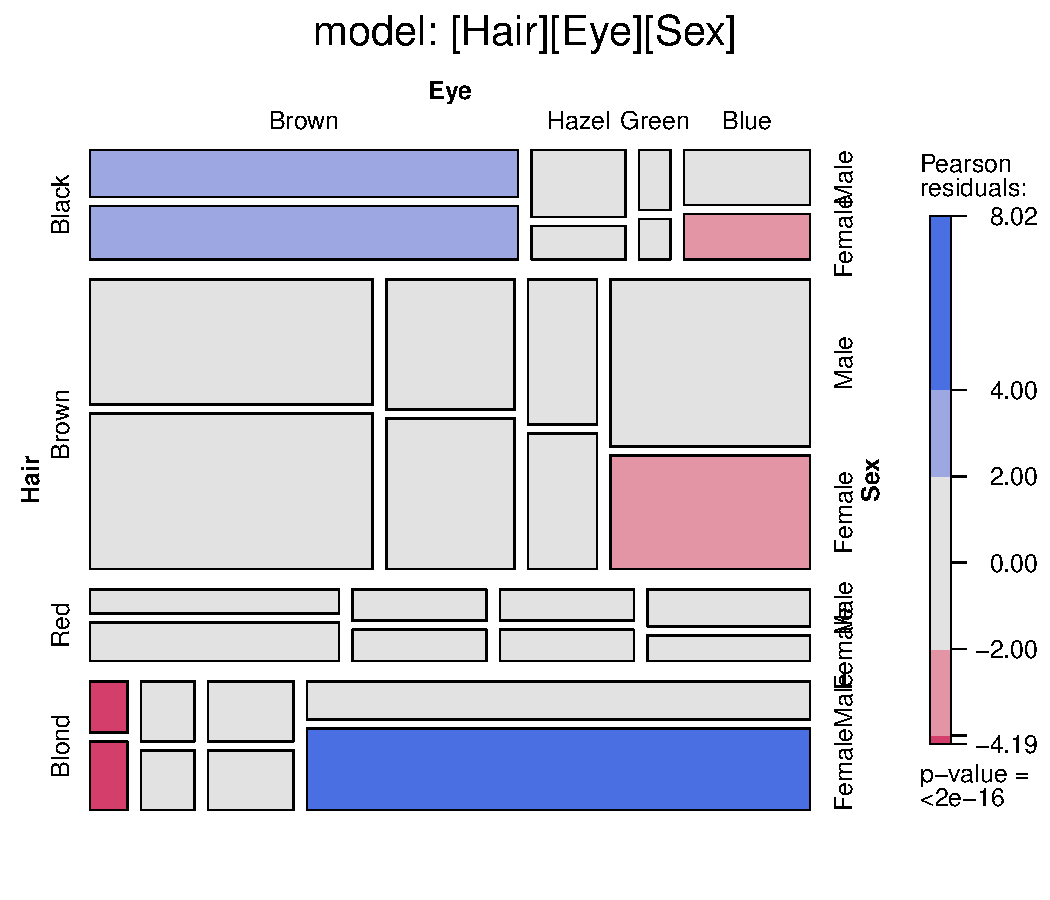
\includegraphics[width=0.32\textwidth]{fig/vcd-tut-hec1}
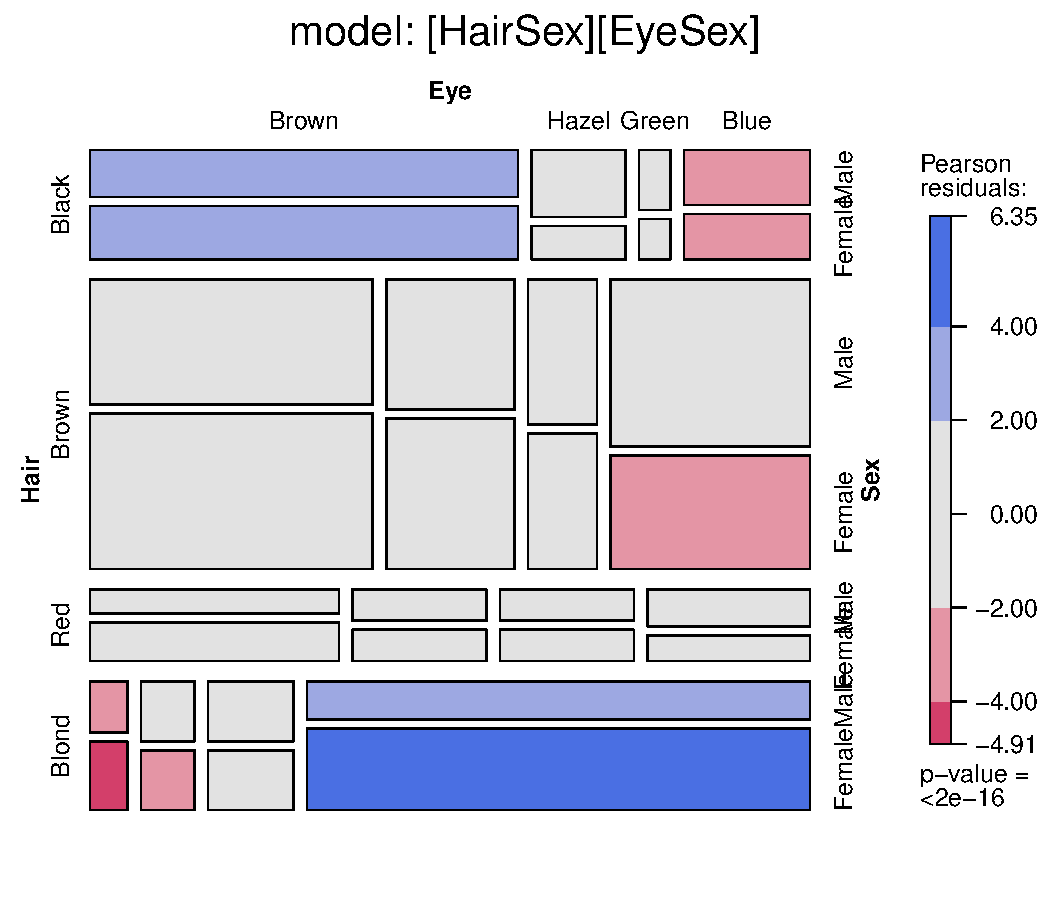
\includegraphics[width=0.32\textwidth]{fig/vcd-tut-hec2}
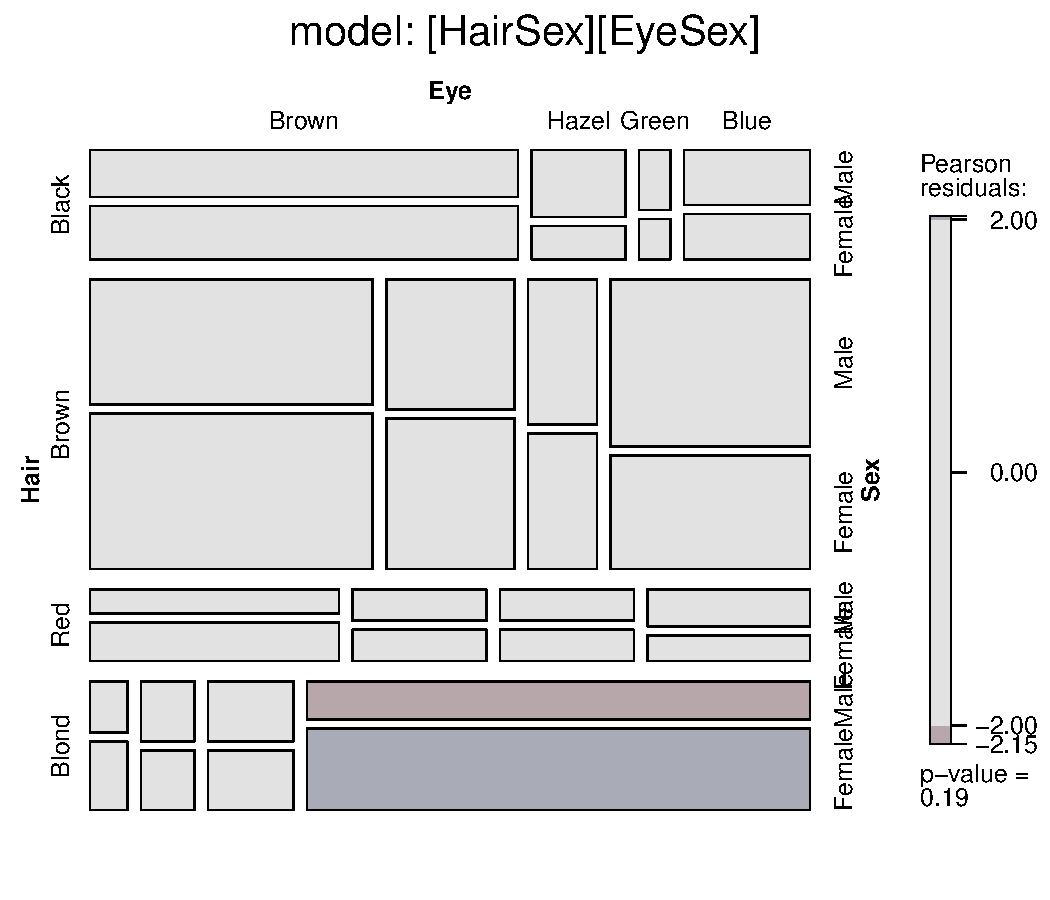
\includegraphics[width=0.32\textwidth]{fig/vcd-tut-hec3}

Alternatively, you can supply the model formula to \codefun{mosaic}
with the \code{expected} argument.  This is passed to \codefun{loglm},
which fits the model, and returns residuals used for shading in the plot. 

For example, here we examine the \data{TV2} constructed in \secref{sec:complex}
above.  The goal is to see how Network choice depends on (varies with)
Day and Time. To do this: 
\begin{itemize}
	\item We fit a model of joint independence of
\code{Network} on the combinations of \code{Day} and \code{Time},
with the model formula \verb|~Day:Time + Network|.
  \item To make the display more easily read, we place \code{Day} and \code{Time}
on the vertical axis and \code{Network} on the horizontal,
  \item The \code{Time} values overlap on the right vertical axis, so we use
  \codefun{level} to abbreviate them.  \codefun{mosaic} also supports a 
  more sophisticated set of labeling functions.  Instead of changing the data
  table, we could have used 
  \verb|labeling_args = list(abbreviate = c(Time = 2))| for a similar effect.
\end{itemize}

The following call to \codefun{mosaic} produces \figref{fig:TV-mosaic}:
\begin{knitrout}
\definecolor{shadecolor}{rgb}{0.969, 0.969, 0.969}\color{fgcolor}\begin{kframe}
\begin{alltt}
\hlkwd{dimnames}\hlstd{(TV2)}\hlopt{$}\hlstd{Time} \hlkwb{<-} \hlkwd{c}\hlstd{(}\hlstr{"8"}\hlstd{,} \hlstr{"9"}\hlstd{,} \hlstr{"10"}\hlstd{)}     \hlcom{# re-level for mosaic display}
\hlkwd{mosaic}\hlstd{(}\hlopt{~} \hlstd{Day} \hlopt{+} \hlstd{Network} \hlopt{+} \hlstd{Time,} \hlkwc{data}\hlstd{=TV2,} \hlkwc{expected}\hlstd{=}\hlopt{~}\hlstd{Day}\hlopt{:}\hlstd{Time} \hlopt{+} \hlstd{Network,}
         \hlkwc{legend}\hlstd{=}\hlnum{FALSE}\hlstd{,} \hlkwc{gp}\hlstd{=shading_Friendly)}
\end{alltt}
\end{kframe}
\end{knitrout}


%\setkeys{Gin}{width=0.75\textwidth}
\begin{figure}[htb]
\begin{center}


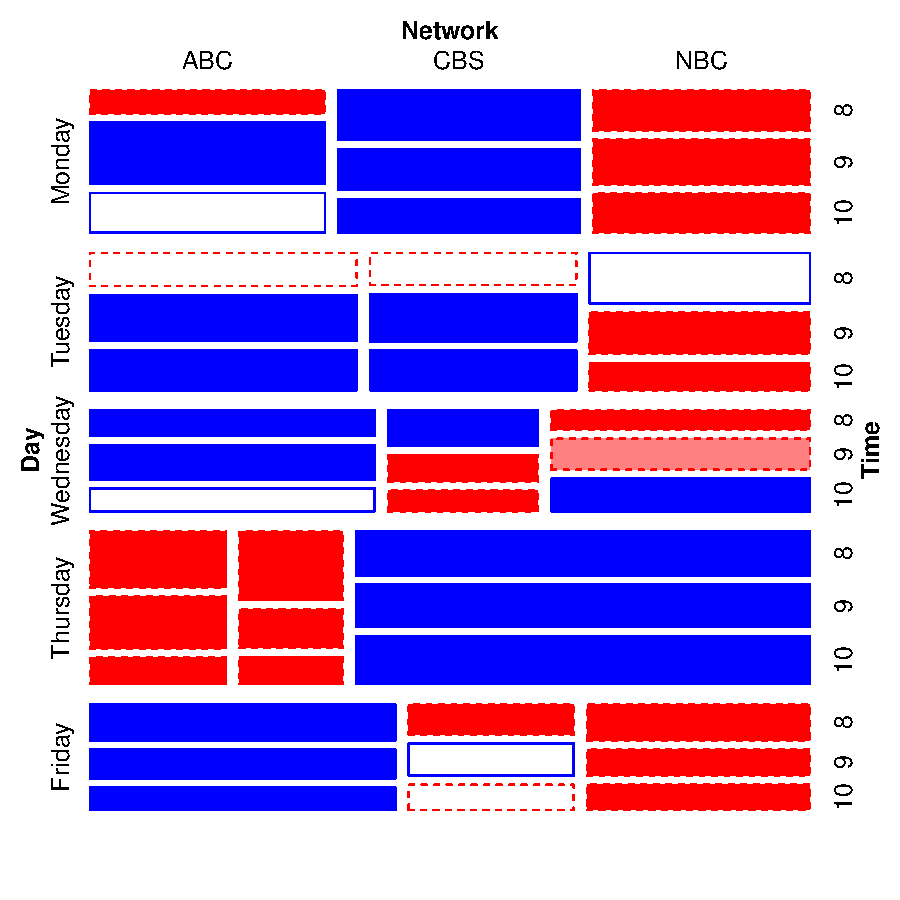
\includegraphics[width=0.75\textwidth,trim=20 30 20 20]{fig/vcd-tut-TV-mosaic}
\caption{Mosaic plot for the \data{TV} data
	showing model of joint independence, \texttt{Day:Time + Network} .}
\label{fig:TV-mosaic}
\end{center}
\end{figure}

From this, it is easy to read from the display how network choice varies with day and
time. For example, CBS dominates in all time slots on Monday;
ABC and NBC dominate on Tuesday, particularly in the later time slots;
Thursday is an NBC day, while on Friday, ABC gets the greatest share.

In interpreting this mosaic and other plots, it is important to understand that
associations included in the model---here, that between day and time---are \emph{not}
shown in the shading of the cells, because they have been fitted (taken into account)
in the \loglin\ model. 

For comparison, you might want to try fitting the model of homogeneous association.
This allows all pairs of factors to be associated, but asserts that each pairwise
association is the same across the levels of the remaining factor.
The resulting plot displays the contributions to a 3-way association, but is not shown here.
\begin{knitrout}
\definecolor{shadecolor}{rgb}{0.969, 0.969, 0.969}\color{fgcolor}\begin{kframe}
\begin{alltt}
\hlkwd{mosaic}\hlstd{(}\hlopt{~} \hlstd{Day} \hlopt{+} \hlstd{Network} \hlopt{+} \hlstd{Time,} \hlkwc{data}\hlstd{=TV2,}
         \hlkwc{expected}\hlstd{=}\hlopt{~}\hlstd{Day}\hlopt{:}\hlstd{Time} \hlopt{+} \hlstd{Day}\hlopt{:}\hlstd{Network} \hlopt{+} \hlstd{Time}\hlopt{:}\hlstd{Network,}
         \hlkwc{legend}\hlstd{=}\hlnum{FALSE}\hlstd{,} \hlkwc{gp}\hlstd{=shading_Friendly)}
\end{alltt}
\end{kframe}
\end{knitrout}


\subsection[Mosaics for glm() and gnm() models]{Mosaics for \codefun{glm} and \codefun{gnm} models}\label{sec:mosglm}
The \pkg{vcdExtra} package provides an additional method, \codefun{mosaic.glm} 
for models fit with \codefun{glm} and \codefun{gnm}.%
\footnote{
Models fit with \codefun{gnm} are of \code{class = c("gnm", "glm", "lm")},
so all \code{*.glm} methods apply, unless overridden in the \pkg{gnm} package.
}
These are not restricted to the 
Poisson family, but only apply to cases where the response variable is non-negative. 

\Example
Here, we plot the independence and the linear-by-linear association model
for the Mental health data from \secref{sec:glm}.
These examples illustrate some of the options for labeling (variable names and
residuals printed in cells).  Note that the \code{formula} supplied to \codefun{mosaic}
for \class{glm} objects refers to the order of factors displayed in the plot, not the model.
\begin{knitrout}
\definecolor{shadecolor}{rgb}{0.969, 0.969, 0.969}\color{fgcolor}\begin{kframe}
\begin{alltt}
\hlstd{long.labels} \hlkwb{<-} \hlkwd{list}\hlstd{(}\hlkwc{set_varnames} \hlstd{=} \hlkwd{c}\hlstd{(}\hlkwc{mental}\hlstd{=}\hlstr{"Mental Health Status"}\hlstd{,} \hlkwc{ses}\hlstd{=}\hlstr{"Parent SES"}\hlstd{))}
\hlkwd{mosaic}\hlstd{(indep,} \hlopt{~}\hlstd{ses}\hlopt{+}\hlstd{mental,} \hlkwc{residuals_type}\hlstd{=}\hlstr{"rstandard"}\hlstd{,}
     \hlkwc{labeling_args} \hlstd{= long.labels,} \hlkwc{labeling}\hlstd{=labeling_residuals,}
     \hlkwc{main}\hlstd{=}\hlstr{"Mental health data: Independence"}\hlstd{)}
\hlkwd{mosaic}\hlstd{(linlin,} \hlopt{~}\hlstd{ses}\hlopt{+}\hlstd{mental,} \hlkwc{residuals_type}\hlstd{=}\hlstr{"rstandard"}\hlstd{,}
     \hlkwc{labeling_args} \hlstd{= long.labels,} \hlkwc{labeling}\hlstd{=labeling_residuals,} \hlkwc{suppress}\hlstd{=}\hlnum{1}\hlstd{,}
     \hlkwc{gp}\hlstd{=shading_Friendly,} \hlkwc{main}\hlstd{=}\hlstr{"Mental health data: Linear x Linear"}\hlstd{)}
\end{alltt}
\end{kframe}
\end{knitrout}


%\setkeys{Gin}{width=0.49\textwidth}





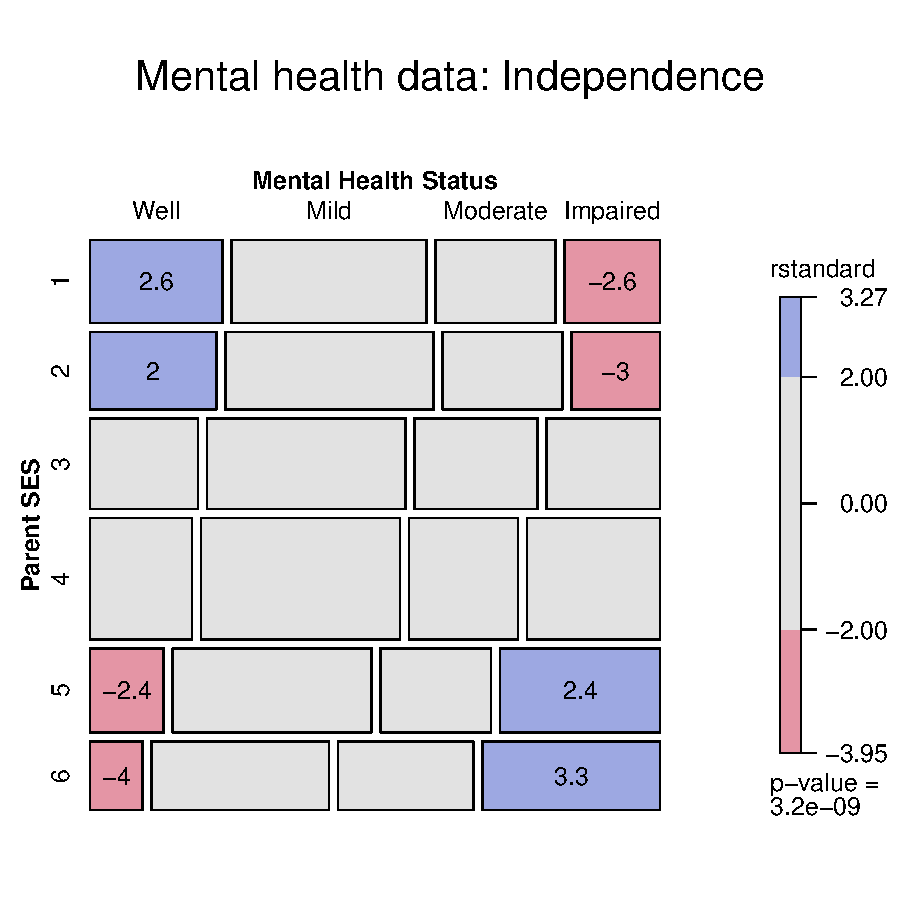
\includegraphics[width=0.49\textwidth]{fig/vcd-tut-mental-plots1}
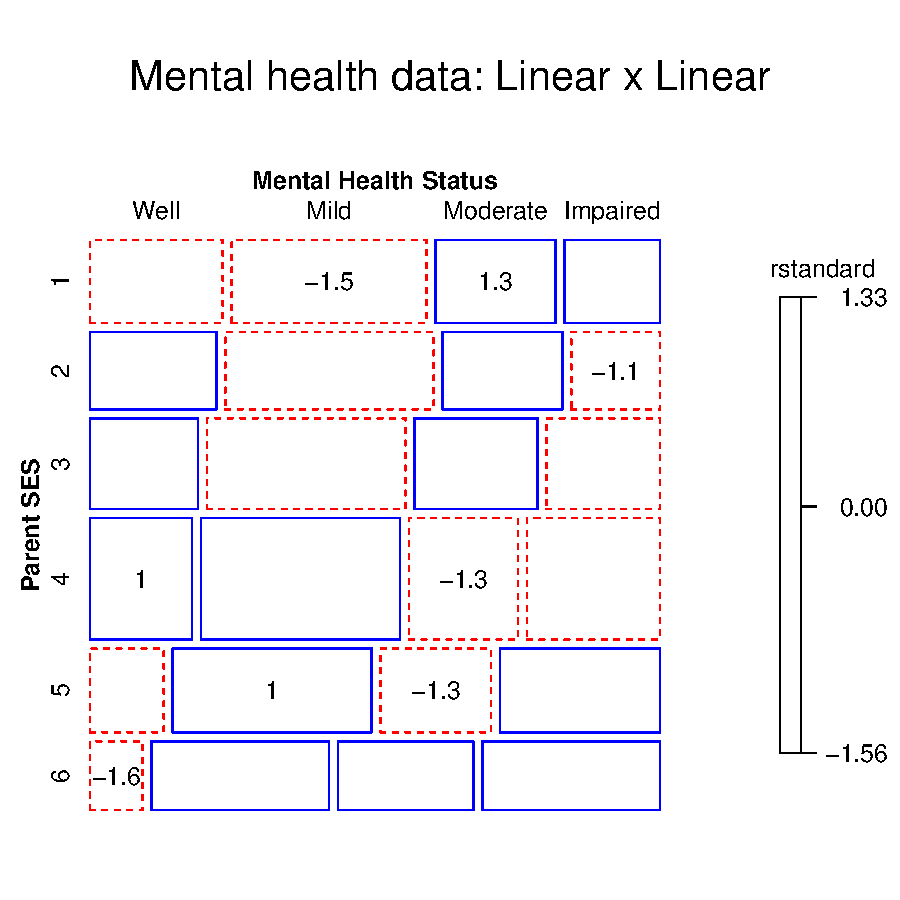
\includegraphics[width=0.49\textwidth]{fig/vcd-tut-mental-plots2}

The \pkg{gnm} package also fits a wide variety of models with nonlinear terms or terms for
structured associations of table variables.  In the following, we fit the RC(1)
model
\begin{equation*}
	\log ( m_{ij} ) = \mu + \lambda_i^A + \lambda_j^B + \phi \mu_i \nu_j 
\end{equation*}
This is similar to the linear by linear model, except that the row effect
parameters ($\mu_i$) and column parameters ($\nu_j$) are estimated from the data
rather than given assigned equally-spaced values.  The multiplicative terms
are specified by the \codefun{Mult}.

\begin{knitrout}
\definecolor{shadecolor}{rgb}{0.969, 0.969, 0.969}\color{fgcolor}\begin{kframe}
\begin{alltt}
\hlstd{Mental}\hlopt{$}\hlstd{mental} \hlkwb{<-} \hlkwd{C}\hlstd{(Mental}\hlopt{$}\hlstd{mental, treatment)}
\hlstd{Mental}\hlopt{$}\hlstd{ses} \hlkwb{<-} \hlkwd{C}\hlstd{(Mental}\hlopt{$}\hlstd{ses, treatment)}
\hlstd{RC1model} \hlkwb{<-} \hlkwd{gnm}\hlstd{(Freq} \hlopt{~} \hlstd{mental} \hlopt{+} \hlstd{ses} \hlopt{+} \hlkwd{Mult}\hlstd{(mental, ses),}
                \hlkwc{family} \hlstd{= poisson,} \hlkwc{data} \hlstd{= Mental)}
\hlkwd{mosaic}\hlstd{(RC1model,} \hlkwc{residuals_type}\hlstd{=}\hlstr{"rstandard"}\hlstd{,} \hlkwc{labeling_args} \hlstd{= long.labels,}
       \hlkwc{labeling}\hlstd{=labeling_residuals,} \hlkwc{suppress}\hlstd{=}\hlnum{1}\hlstd{,} \hlkwc{gp}\hlstd{=shading_Friendly,}
       \hlkwc{main}\hlstd{=}\hlstr{"Mental health data: RC(1) model"}\hlstd{)}
\end{alltt}
\end{kframe}
\end{knitrout}

Other forms of nonlinear terms are provided for the inverse of a predictor
(\codefun{Inv}) and the exponential of a predictor (\codefun{Exp}).
You should read \code{vignette("gnmOverview", package="gnm")} for further details.

\subsection{Mosaic tips and techniques}\label{sec:tips}

The \pkg{vcd} package implements an extremely general collection of graphical methods for
$n$-way frequency tables within the strucplot framework, which includes mosaic plots
(\codefun{mosaic}), as well as association plots (\codefun{assoc}), sieve diagrams
(\codefun{sieve}), as well as tabular displays (\codefun{structable}).

The graphical methods in \pkg{vcd}  support a wide of options that control almost all of the details
of the plots, but it is often difficult to determine what arguments you need to supply
to achieve a given effect from the \code{help()}.  As a first step, you should read the 
\code{vignette("strucplot")} in \pkg{vcd} to understand the overall structure of
these plot methods.  The notes below describe a few useful things that may not be obvious,
or can be done in different ways.

\subsubsection[Changing labels]{Changing the labels for variables and levels}
With data in contingency table form or as a frequency data frame, it often happens
that the variable names and/or the level values of the factors, while suitable
for analysis, are less than adequate when used in mosaic plots and other strucplot
displays.  

For example, we might prefer that a variable named \code{ses} appear
as \code{"Socioeconomic Status"}, or a factor with levels \code{c("M", "F")}
be labeled using \code{c("Male", "Female")} in a plot.  Or, sometimes we
start with a factor whose levels are fully spelled out
(e.g., \code{c("strongly disagree", "disagree", "neutral", "agree", "strongly agree")}),
only to find that the level labels overlap in graphic displays.

The structplot framework in \pkg{vcd} provides an extremely large variety of
functions and options for controlling almost all details of text labels in mosaics
and other plots.  See \code{help(labelings)} for an overview. 

For example, in \secref{sec:ordered-factors} we showed how to rearrange the dimensions
of the \code{UCBAdmissions} table, change the names of the table variables, and
relabel the levels of one of the table variables.
The code below changes the actual table for plotting purposes, but we pointed out that
these changes can create other problems in analysis.

\begin{knitrout}
\definecolor{shadecolor}{rgb}{0.969, 0.969, 0.969}\color{fgcolor}\begin{kframe}
\begin{alltt}
\hlstd{UCB} \hlkwb{<-} \hlkwd{aperm}\hlstd{(UCBAdmissions,} \hlkwd{c}\hlstd{(}\hlnum{2}\hlstd{,} \hlnum{1}\hlstd{,} \hlnum{3}\hlstd{))}
\hlkwd{names}\hlstd{(}\hlkwd{dimnames}\hlstd{(UCB))} \hlkwb{<-} \hlkwd{c}\hlstd{(}\hlstr{"Sex"}\hlstd{,} \hlstr{"Admit?"}\hlstd{,} \hlstr{"Department"}\hlstd{)}
\hlkwd{dimnames}\hlstd{(UCB)[[}\hlnum{2}\hlstd{]]} \hlkwb{<-} \hlkwd{c}\hlstd{(}\hlstr{"Yes"}\hlstd{,} \hlstr{"No"}\hlstd{)}
\end{alltt}
\end{kframe}
\end{knitrout}


The same effects can be achieved \emph{without} modifying the data
using the \verb|set_varnames| and
\verb|set_labels| options in \codefun{mosaic} as follows:

\begin{knitrout}
\definecolor{shadecolor}{rgb}{0.969, 0.969, 0.969}\color{fgcolor}\begin{kframe}
\begin{alltt}
\hlstd{vnames} \hlkwb{<-} \hlkwd{list}\hlstd{(}\hlkwc{set_varnames} \hlstd{=} \hlkwd{c}\hlstd{(}\hlkwc{Admit}\hlstd{=}\hlstr{"Admission"}\hlstd{,} \hlkwc{Gender}\hlstd{=}\hlstr{"Sex"}\hlstd{,} \hlkwc{Dept}\hlstd{=}\hlstr{"Department"}\hlstd{))}
\hlstd{lnames} \hlkwb{<-} \hlkwd{list}\hlstd{(}\hlkwc{Admit} \hlstd{=} \hlkwd{c}\hlstd{(}\hlstr{"Yes"}\hlstd{,} \hlstr{"No"}\hlstd{),}
              \hlkwc{Gender} \hlstd{=} \hlkwd{c}\hlstd{(}\hlstr{"Males"}\hlstd{,} \hlstr{"Females"}\hlstd{),}
              \hlkwc{Dept} \hlstd{= LETTERS[}\hlnum{1}\hlopt{:}\hlnum{6}\hlstd{])}
\hlkwd{mosaic}\hlstd{(UCBAdmissions,} \hlkwc{labeling_args}\hlstd{=vnames,} \hlkwc{set_labels}\hlstd{=lnames)}
\end{alltt}
\end{kframe}
\end{knitrout}


In some cases, it may be sufficient to abbreviate (or clip, or rotate) level names to avoid 
overlap.  For example, the statements below produce another version of
\figref{fig:TV-mosaic} with days of the week abbreviated to their first three letters.
Section 4 in the \code{vignette("strucplot")} provides many other examples.

\begin{knitrout}
\definecolor{shadecolor}{rgb}{0.969, 0.969, 0.969}\color{fgcolor}\begin{kframe}
\begin{alltt}
\hlkwd{dimnames}\hlstd{(TV2)}\hlopt{$}\hlstd{Time} \hlkwb{<-} \hlkwd{c}\hlstd{(}\hlstr{"8"}\hlstd{,} \hlstr{"9"}\hlstd{,} \hlstr{"10"}\hlstd{)}     \hlcom{# re-level for mosaic display}
\hlkwd{mosaic}\hlstd{(}\hlopt{~} \hlstd{Day} \hlopt{+} \hlstd{Network} \hlopt{+} \hlstd{Time,} \hlkwc{data}\hlstd{=TV2,} \hlkwc{expected}\hlstd{=}\hlopt{~}\hlstd{Day}\hlopt{:}\hlstd{Time} \hlopt{+} \hlstd{Network,}
         \hlkwc{legend}\hlstd{=}\hlnum{FALSE}\hlstd{,} \hlkwc{gp}\hlstd{=shading_Friendly,}
         \hlkwc{labeling_args}\hlstd{=}\hlkwd{list}\hlstd{(}\hlkwc{abbreviate}\hlstd{=}\hlkwd{c}\hlstd{(}\hlkwc{Day}\hlstd{=}\hlnum{3}\hlstd{)) )}
\end{alltt}
\end{kframe}
\end{knitrout}


%\subsubsection{Fitting complex models with glm() and gnm()}



\section[Continuous predictors]{Continuous predictors}\label{sec:contin}
When continuous predictors are available---and potentially important--- in explaining a
categorical outcome, models for that outcome include:
logistic regression (binary response), 
the proportional odds model (ordered polytomous response),
multinomial (generalized) logistic regression.
Many of these are special cases of the generalized linear model using the
\code{"poisson"} or \code{"binomial"} family and their relatives.

\subsection{Spine and conditional density plots}\label{sec:spine}
I don't go into fitting such models here, but I would be remiss not to illustrate some
visualizations in \pkg{vcd} that are helpful here.
The first of these is the spine plot or spinogram \citep{vcd:Hummel:1996}
 (produced with \codefun{spine}).
These are special cases of mosaic plots with 
specific spacing and shading to show how a categorical response varies with
a continuous or categorical predictor.

They are also a generalization of stacked bar plots where not the heights  but
the \emph{widths} of the bars corresponds to the relative frequencies of \code{x}. The heights
of the  bars then  correspond to  the conditional  relative frequencies  of {y} in
every \code{x} group.

\Example
For the \data{Arthritis} data, we can see how \code{Improved} varies with \code{Age}
as follows.  \codefun{spine} takes a formula of the form 
\verb|y ~ x| with a single dependent factor and a single explanatory variable \code{x}
(a numeric variable or a factor).
The range of a numeric variable\code{x} is divided into intervals based on the
\code{breaks} argument, and stacked bars are drawn to show the distribution of
\code{y} as \code{x} varies.  As shown below, the discrete table that is visualized
is returned by the function.

\begin{knitrout}
\definecolor{shadecolor}{rgb}{0.969, 0.969, 0.969}\color{fgcolor}\begin{kframe}
\begin{alltt}
\hlstd{(}\hlkwd{spine}\hlstd{(Improved} \hlopt{~} \hlstd{Age,} \hlkwc{data} \hlstd{= Arthritis,} \hlkwc{breaks} \hlstd{=} \hlnum{3}\hlstd{))}
\end{alltt}
\begin{verbatim}
##          Improved
## Age       None Some Marked
##   [20,40]   10    3      2
##   (40,60]   21    3     17
##   (60,80]   11    8      9
\end{verbatim}
\begin{alltt}
\hlstd{(}\hlkwd{spine}\hlstd{(Improved} \hlopt{~} \hlstd{Age,} \hlkwc{data} \hlstd{= Arthritis,} \hlkwc{breaks} \hlstd{=} \hlstr{"Scott"}\hlstd{))}
\end{alltt}
\begin{verbatim}
##          Improved
## Age       None Some Marked
##   [20,30]    6    1      0
##   (30,40]    4    2      2
##   (40,50]    9    0      3
##   (50,60]   12    3     14
##   (60,70]   11    8      8
##   (70,80]    0    0      1
\end{verbatim}
\end{kframe}
\end{knitrout}


\setkeys{Gin}{width=0.49\textwidth}






The conditional density plot \citep{vcd:Hofmann+Theus} is a further generalization.
This visualization technique is similar to spinograms, but uses a smoothing approach
rather than discretizing the explanatory variable.  As well, it uses 
the original \code{x} axis and not a distorted one.

%\setkeys{Gin}{width=0.6\textwidth}
\begin{figure}[htb]
\begin{center}
\begin{knitrout}
\definecolor{shadecolor}{rgb}{0.969, 0.969, 0.969}\color{fgcolor}\begin{kframe}
\begin{alltt}
\hlkwd{cdplot}\hlstd{(Improved} \hlopt{~} \hlstd{Age,} \hlkwc{data} \hlstd{= Arthritis)}
\hlkwd{with}\hlstd{(Arthritis,} \hlkwd{rug}\hlstd{(}\hlkwd{jitter}\hlstd{(Age),} \hlkwc{col}\hlstd{=}\hlstr{"white"}\hlstd{,} \hlkwc{quiet}\hlstd{=}\hlnum{TRUE}\hlstd{))}
\end{alltt}
\end{kframe}
\end{knitrout}

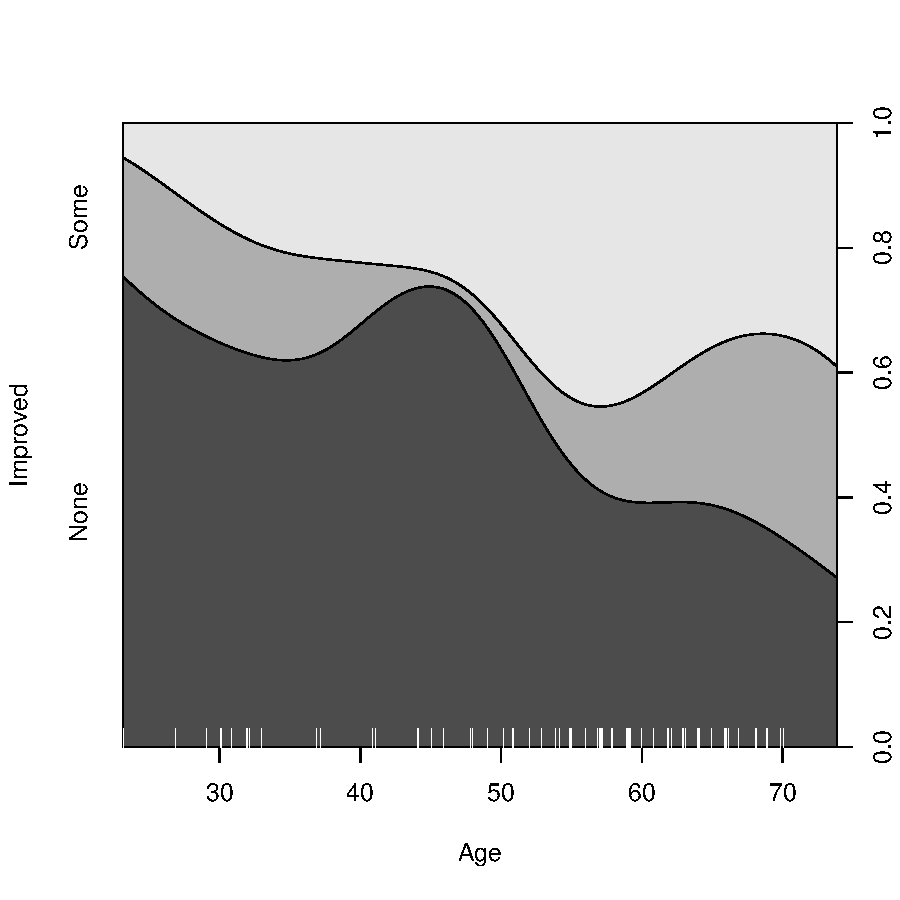
\includegraphics[width=0.6\textwidth]{fig/vcd-tut-cdplot}
\caption{Conditional density plot for the \data{Arthritis} data
	showing the variation of Improved with Age.}
\label{fig:cd-plot}
\end{center}
\end{figure}

In such plots, it is useful to also see the distribution of the observations
across the horizontal axis, e.g., with a \codefun{rug} plot.
\figref{fig:cd-plot} uses \codefun{cdplot} from the \pkg{graphics} package
rather than \verb|cd_plot()| from \pkg{vcd}, and is produced with
\begin{knitrout}
\definecolor{shadecolor}{rgb}{0.969, 0.969, 0.969}\color{fgcolor}\begin{kframe}
\begin{alltt}
\hlkwd{cdplot}\hlstd{(Improved} \hlopt{~} \hlstd{Age,} \hlkwc{data} \hlstd{= Arthritis)}
\hlkwd{with}\hlstd{(Arthritis,} \hlkwd{rug}\hlstd{(}\hlkwd{jitter}\hlstd{(Age),} \hlkwc{col}\hlstd{=}\hlstr{"white"}\hlstd{,} \hlkwc{quiet}\hlstd{=}\hlnum{TRUE}\hlstd{))}
\end{alltt}
\end{kframe}
\end{knitrout}

From \figref{fig:cd-plot} it can be easily seen that the proportion
of patients reporting Some or Marked improvement increases with Age,
but there are some peculiar bumps in the distribution.
These may be real or artifactual, but they would be hard to see
with most other visualization methods.
When we switch from non-parametric data exploration to parametric
statistical models, such effects are easily missed.

\subsection[Model-based plots]{Model-based plots: effect plots and \pkg{ggplot2} plots}\label{sec:modelplots}
The nonparametric conditional density plot uses smoothing methods
to convey the distributions of the response variable,
but displays that are simpler to interpret can often be obtained by plotting
the predicted response from a parametric model.

For complex \codefun{glm} models with interaction effects, the \pkg{effects}
package  provides the most useful displays,
plotting  the predicted values for a given term, averaging over other
predictors not included in that term.  I don't illustrate this here, but
see \citet{effects:1,effects:2} and \code{help(package="effects")}.

Here I just briefly illustrate the capabilities of the \pkg{ggplot2} package
for model-smoothed plots of categorical responses in \codefun{glm} models.

\Example
The \data{Donner} data frame in \pkg{vcdExtra} gives details on the survival
of 90 members of the Donner party,
a group of people who attempted to migrate to California in 1846.
They were trapped by an early blizzard on the eastern side of the
Sierra Nevada mountains, and before they could be rescued, 
nearly half of the party had died.
What factors affected who lived and who died?

\begin{knitrout}
\definecolor{shadecolor}{rgb}{0.969, 0.969, 0.969}\color{fgcolor}\begin{kframe}
\begin{alltt}
\hlkwd{data}\hlstd{(Donner,} \hlkwc{package}\hlstd{=}\hlstr{"vcdExtra"}\hlstd{)}
\hlkwd{str}\hlstd{(Donner)}
\end{alltt}
\begin{verbatim}
## 'data.frame':	90 obs. of  5 variables:
##  $ family  : Factor w/ 10 levels "Breen","Donner",..: 9 1 1 1 1 1 1 1 1 1 ...
##  $ age     : int  23 13 1 5 14 40 51 9 3 8 ...
##  $ sex     : Factor w/ 2 levels "Female","Male": 2 2 1 2 2 1 2 2 2 2 ...
##  $ survived: int  0 1 1 1 1 1 1 1 1 1 ...
##  $ death   : POSIXct, format: "1846-12-29" NA ...
\end{verbatim}
\end{kframe}
\end{knitrout}

A potential model of interest
is the logistic regression model for $Pr(survived)$, allowing separate
fits for males and females as a function of \code{age}.
The key to this is the \verb|stat_smooth()| function, using
	\code{method = "glm", family = binomial}. The \verb|formula = y ~ x|
	specifies a linear fit on the logit scale (\figref{fig:donner3}, left)

\begin{knitrout}
\definecolor{shadecolor}{rgb}{0.969, 0.969, 0.969}\color{fgcolor}\begin{kframe}
\begin{alltt}
\hlcom{# separate linear fits on age for M/F}
\hlkwd{ggplot}\hlstd{(Donner,} \hlkwd{aes}\hlstd{(age, survived,} \hlkwc{color} \hlstd{= sex))} \hlopt{+}
  \hlkwd{geom_point}\hlstd{(}\hlkwc{position} \hlstd{=} \hlkwd{position_jitter}\hlstd{(}\hlkwc{height} \hlstd{=} \hlnum{0.02}\hlstd{,} \hlkwc{width} \hlstd{=} \hlnum{0}\hlstd{))} \hlopt{+}
  \hlkwd{stat_smooth}\hlstd{(}\hlkwc{method} \hlstd{=} \hlstr{"glm"}\hlstd{,} \hlkwc{family} \hlstd{= binomial,} \hlkwc{formula} \hlstd{= y} \hlopt{~} \hlstd{x,}
           \hlkwc{alpha} \hlstd{=} \hlnum{0.2}\hlstd{,} \hlkwc{size}\hlstd{=}\hlnum{2}\hlstd{,} \hlkwd{aes}\hlstd{(}\hlkwc{fill} \hlstd{= sex))}
\end{alltt}
\end{kframe}
\end{knitrout}

Alternatively, we can allow a quadratic relation with \code{age}
by specifying \verb|formula = y ~ poly(x,2)| (\figref{fig:donner3}, right).
\begin{knitrout}
\definecolor{shadecolor}{rgb}{0.969, 0.969, 0.969}\color{fgcolor}\begin{kframe}
\begin{alltt}
\hlcom{# separate quadratics}
\hlkwd{ggplot}\hlstd{(Donner,} \hlkwd{aes}\hlstd{(age, survived,} \hlkwc{color} \hlstd{= sex))} \hlopt{+}
  \hlkwd{geom_point}\hlstd{(}\hlkwc{position} \hlstd{=} \hlkwd{position_jitter}\hlstd{(}\hlkwc{height} \hlstd{=} \hlnum{0.02}\hlstd{,} \hlkwc{width} \hlstd{=} \hlnum{0}\hlstd{))} \hlopt{+}
  \hlkwd{stat_smooth}\hlstd{(}\hlkwc{method} \hlstd{=} \hlstr{"glm"}\hlstd{,} \hlkwc{family} \hlstd{= binomial,} \hlkwc{formula} \hlstd{= y} \hlopt{~} \hlkwd{poly}\hlstd{(x,}\hlnum{2}\hlstd{),}
           \hlkwc{alpha} \hlstd{=} \hlnum{0.2}\hlstd{,} \hlkwc{size}\hlstd{=}\hlnum{2}\hlstd{,} \hlkwd{aes}\hlstd{(}\hlkwc{fill} \hlstd{= sex))}
\end{alltt}
\end{kframe}
\end{knitrout}


%\setkeys{Gin}{width=0.49\textwidth}
\begin{figure}[htb]
\begin{center}




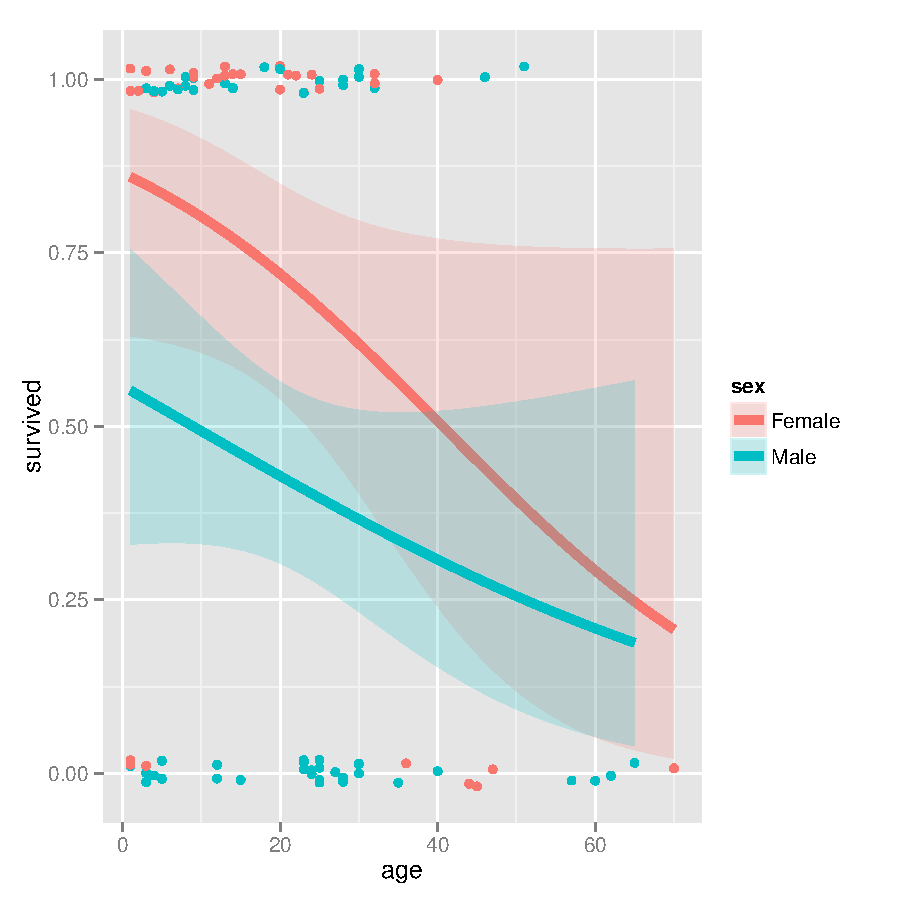
\includegraphics[width=0.49\textwidth]{fig/vcd-tut-donner3a}
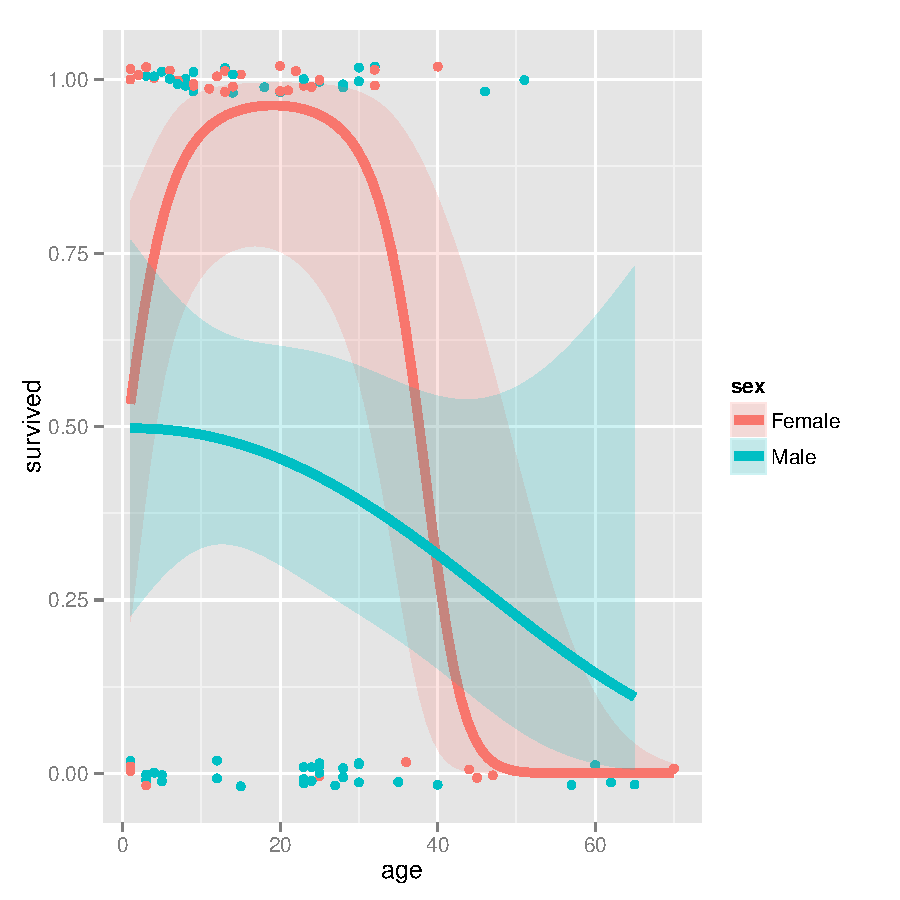
\includegraphics[width=0.49\textwidth]{fig/vcd-tut-donner3b}
\caption{Logistic regression plots for the  \data{Donner} data
	showing survival vs. age, by sex. Left: linear logistic model; right: quadratic model}
\label{fig:donner3}
\end{center}
\end{figure}
These plots very nicely show (a) the fitted $Pr(survived)$ for males and females;
(b) confidence bands around the smoothed model fits and (c) the individual
observations by jittered points at 0 and 1 for those who died and survided, respectively.

\bibliography{vcd,vcdExtra}

\end{document}
